%!TEX root = ../thesis.tex
%*******************************************************************************
%*********************************** Second Chapter *****************************
%*******************************************************************************
\cleardoublepage
\chapter{Introduction to wind turbine modeling and design}
\label{chpt:2}
%*******************************************************************************
\hfill
\localtableofcontents
\newpage

%============================================================%
%============================================================%
\section{Introduction}
%============================================================%
%============================================================%

Wind energy is a highly competitive industry with increasing regulations regarding its impact on ecosystems, land and sea use, landscapes, or air traffic management \citep{eolien_en_mer_2022}. 
During the long process of winning calls for tenders, obtaining construction permits, or through wind farm exploitation, an advanced technical understanding of such systems might offer a competitive advantage. 

The operation of offshore wind turbines (OWTs) is driven by multiple coupled physics. 
This behavior results from different external loading which are highly turbulent and uncertain. 
Among them, the \textit{metocean} (abbreviation of ``meteorology'' and ``oceanography'') environmental conditions play a primary role. 
Yet, many other types of solicitations affect the exploitation of offshore wind turbines such as the corrosion of the structure, global scour, marine growth, stress concentration factor induced by the manufacturing process, etc. 

In this context, numerical models have been developed to certify the structural integrity of OWTs w.r.t. external solicitations. 
A wind farm project planned at a given location should pass different validation procedures (regarding fatigue, ultimate loads, buckling, serviceability, etc.) established by international standards such as the International Electrotechnical Commission \citep{iec_2019}. 
As wind turbine structures face a large number of stress cycles in their lifetime (up to $10^8$ for 25 years of operation), this chapter will particularly focus on fatigue damage assessment.

The present thesis studied different steps of the UQ methodology on two wind farm projects. 
First, the Teesside wind farm, operating since 2014 in the North Sea, second the theoretical wind farm of south Brittany, currently at the stage of calls for tenders.

Considering the standard UQ methodology presented in \fig{fig:UQ_methodo}, the material of this chapter is related to step A (problem specification) and step B (quantification of sources of uncertainty). 
It briefly introduces wind turbine modeling and design, in the following layout: 
Section~\ref{sec:metocean_simulation} presents the methods used for wind and wave generation and wake simulation at a farm scale; 
Section~\ref{sec:owt_modeling} recalls elements of theory associated with wind turbine modeling; 
Section~\ref{sec:owt_design} introduces recommended practices regarding design and operation; 
finally, Section~\ref{sec:owt_uncertainties} describes the various sources of uncertainties considered in this thesis. 
%To go further this general introduction, the reader might refer to the following sources on the different topics 



%============================================================%
%============================================================%
\section{Metocean conditions simulation} \label{sec:metocean_simulation}
%============================================================%
%============================================================%

In the atmosphere, the wind represents the air movements caused by the heterogeneous solar heating of Earth's surface. 
Winds usually move from high-pressure to low-pressure regions. 
Earth's rotation also impacts large-scale climate patterns, including winds by the intermediate of the well-known Coriolis effect. 
The wind is a highly variable resource, making its exploitation for energy production uncertain. 
This variability is expressed in space and time with different behaviors depending on the scales studied. 

Regarding large timescales, yearly seasonal fluctuations of wind conditions are well-defined using probability distributions (typically, Weibull distributions \citealp{burton_2021_wind_handbook}). 
However, predictions at a shorter timescale are usually unreliable beyond a few days ahead. 
Under a few days, the spectral wind energy distribution per time unit is represented by its power spectral density. 
Historically, the spectral study of horizontal wind by \citet{van_1957_wind_psd} for timescales between a few seconds and ten days revealed distinct ranges of behaviors. 
The power spectral density, such as the one illustrated in \fig{fig:wind_psd}, presents three main separated peaks, explaining how the wind energy is split. 
The two first peaks are named ``synoptic'' and ``diurnal'' peaks, which respectively correspond to return periods around four days and one day. 
While these two peaks are relatively close together, the third peak is completely separated. 
This third peak describes the energy related to wind turbulence, which evolves in a range below ten minutes. 
Considering this typical energy distribution, wind behaviors are often referred to as ``short-term'' (for turbulent wind) and ``long-term'' (otherwise). 
In bottom-fixed wind turbine simulation, ten-minute simulations became a common practice to fully consider turbulent winds. 

Remark that the spectrum presented in the paper of \citet{van_1957_wind_psd} (represented in \fig{fig:wind_psd}) was built from wind measures near New York, USA. 
The same pattern between the three peaks is rather constant between sites, however, the geography (including the surface roughness, the topology, the proximity to the coast, etc.) may affect this distribution. 

At a larger timescale than one year, assessing trends becomes more complicated. 
Additionally, wind resource assessment over decades is made more uncertain by climate change (see \citealp{nagababu_2023_climate_change}), disrupting large weather trends and increasing the occurrence of extreme events. 

\begin{figure}
    \centering
    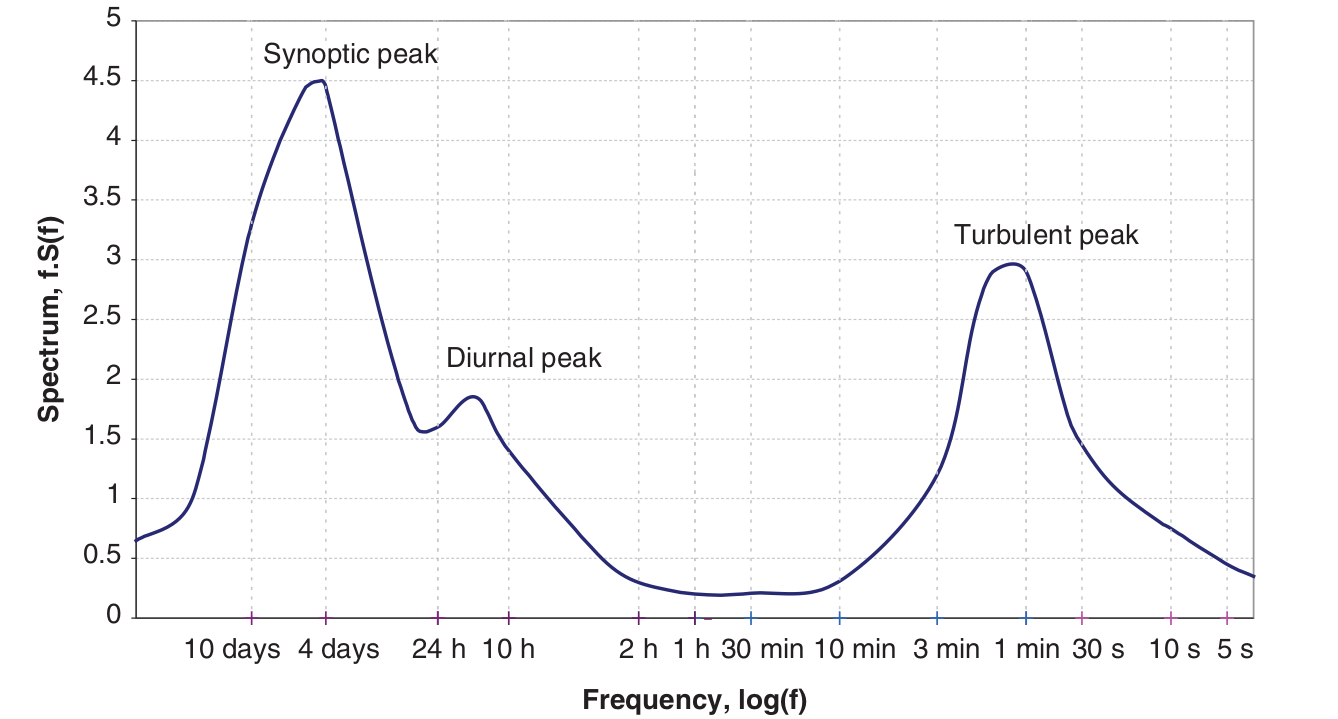
\includegraphics[width=0.7\textwidth]{./part1/figures/wind_spectrum.png}
    \caption{Wind power spectral density from Brookhaven, USA (source: \citealp{burton_2021_wind_handbook}).}
    \label{fig:wind_psd}
\end{figure}





%============================================================%
\subsection{Turbulent wind generation}\label{sec:221}
%============================================================%

Wind turbulence is a complex and aleatory process, often described as chaotic, since a small perturbation of its initial conditions might have a large impact on the response. 
However, the wind over short-term periods (i.e., ten minutes periods) is usually assumed to be a Gaussian process with constant mean $\overline{U}$ and standard deviation $\sigma_U$ \citep{burton_2021_wind_handbook}. 
Its mean is modeled by the long-term wind conditions (i.e., mean wind speed), often described by a probabilistic model such as a Weibull distribution. 
%\elias{This short-term / long-term modeling hypothesis is represented in \fig{fig:wind_long_short_term}.} 
Note that this assumption is based on the bimodal wind energy distribution observed in \fig{fig:wind_psd}, which might vary at some specific locations. 
A discussion on the Gaussian hypothesis for turbulent wind generation is proposed in \citet[Sec. 7]{hiperwind_2022_wp31}.

The \textit{turbulence intensity} is a commonly used normalized statistic of the wind variability: 
\begin{equation}
    I = \frac{\sigma_U}{\overline{U}}.
\end{equation}

%\begin{figure}
%    \centering
%    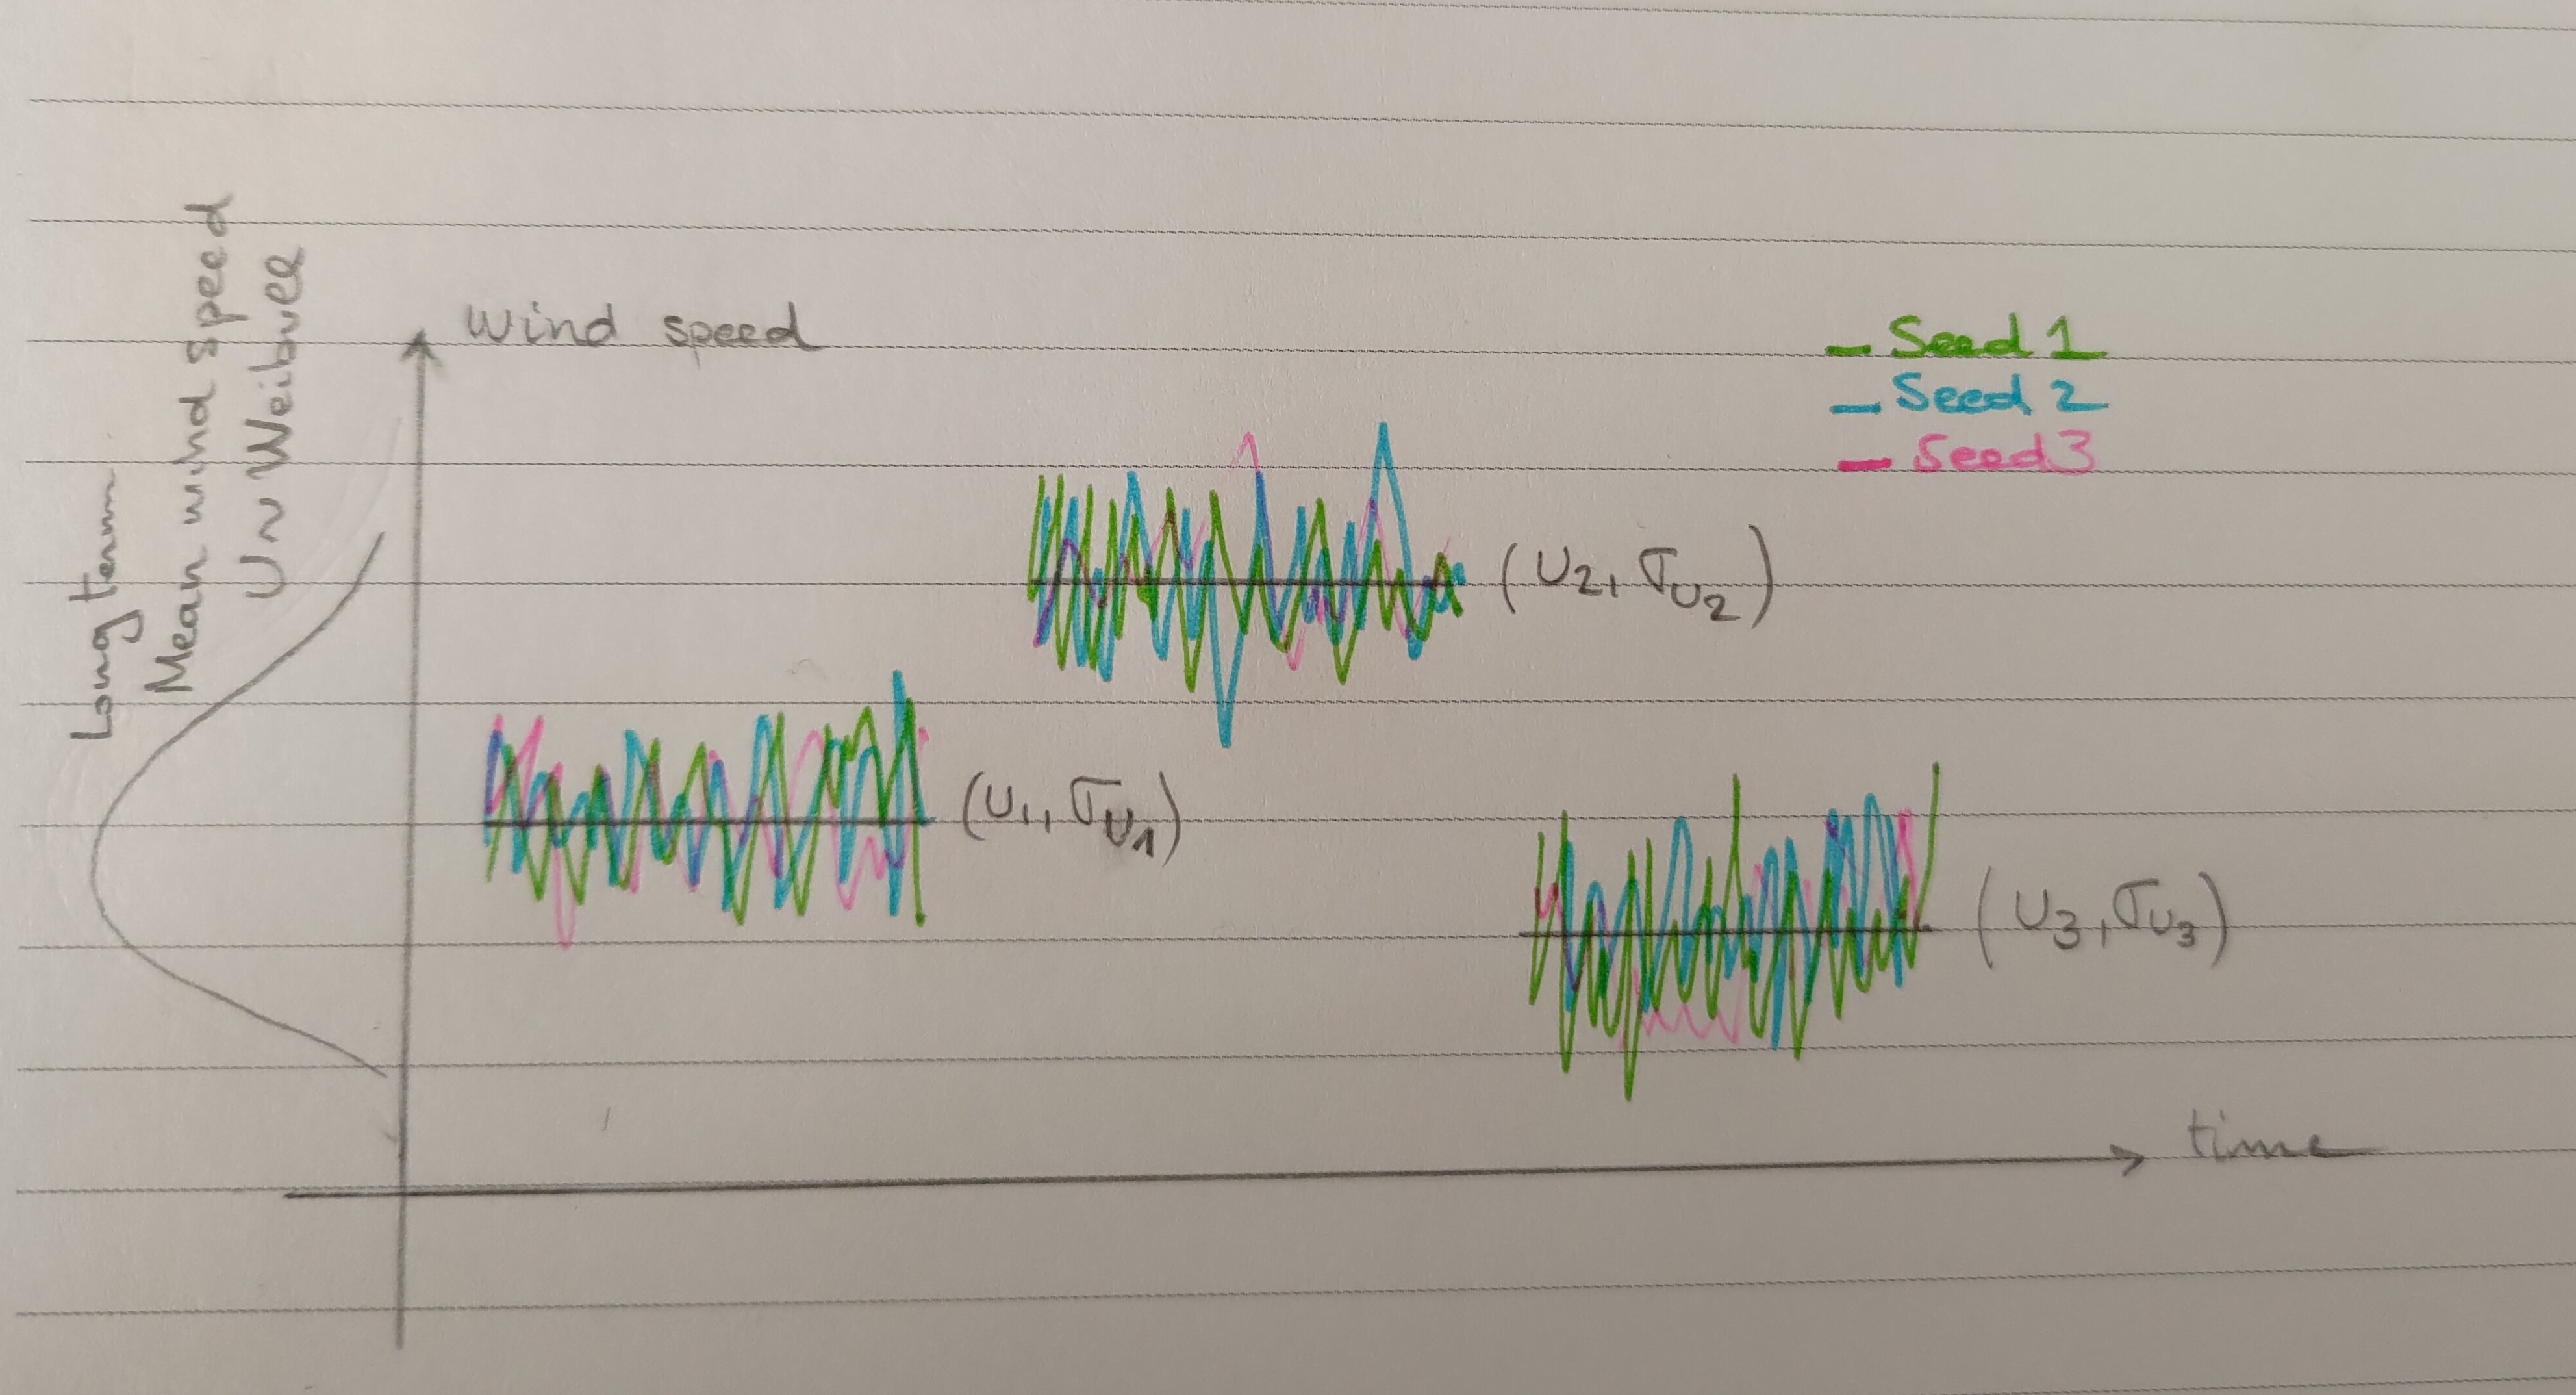
\includegraphics[width=0.7\textwidth]{./part1/figures/wind_long_short_term.jpg}
%    \label{fig:wind_long_short_term}
%    \caption{\elias{Should we keep this representation? If so, it will be done properly.}}
%\end{figure}

As the wind depends on differences between pressure, humidity, and air density, different models exist to represent vertical wind profiles. 
The vertical change in wind conditions is referred to as \textit{vertical wind shear}. 
Assuming a constant standard deviation over the altitude $z$, the power law is a widely used model to approximate vertical shear \citep{iec_2019}:
\begin{equation}
    \overline{U}(z) = \overline{U}_0 \left(\frac{z}{z_{\mathrm{0}}}\right)^\alpha,
\end{equation}
where $\overline{U}_0$ is a well-defined mean wind speed at the height $z_{\mathrm{0}}$ (typically corresponding to a specific measurement height), 
$z$ is the studied height (e.g., the turbine's hub height), and $\alpha$ is the vertical shear coefficient (defined according to measures or standards' recommendations). 

To generate a turbulent wind field on a mesh around the turbine, the general mechanism is to apply inverse Fourier transforms on a turbulent wind spectrum.  
Two types of parametric spectrums are commonly used in wind energy: the \textit{Kaimal model} \citep{kaimal_1972} and the \textit{Mann model} \citep{mann_1998}. 
In this thesis, the Kaimal spectrum as defined in \cite{iec_2019} is used for turbulent wind generation over the Cartesian component $k \in \{u, v, w\}$:
\begin{equation}
    S_k(f) = \frac{4 \sigma_k^2 \frac{L_k}{\overline{U}}}{\left(1 + 6 f \frac{L_k}{\overline{U}}\right)^{5/3}},
    \label{eq:kaimal}
\end{equation} 
such that $f$ is the frequency, $\overline{U}$ is the longitudinal mean speed at hub-height, $L_k$ are the Kaimal length scales, and $\sigma_k$ standard deviations. 
Along with the Kaimal wind speed spectrum, a spatial coherence model is usually defined in the frequency domain. 
Each couple of nodes in the mesh are correlated, for example, using an exponential coherence model (see the complete definition in \citealp[Appendix C]{iec_2019}).

In this thesis, the full-field turbulent wind fields (i.e., over a regular mesh) are generated using TurbSim, a software developed by the National Renewable Energy Laboratory (NREL) \citep{turbsim_2009}. 
TurbSim generates time realizations by adapting the spectral method proposed in \citet{veers_1988_sandia} (relying on the inverse Fourier transforms of each axial component).   
Considering a wind spectrum (e.g., Kaimal model) and a vertical shear model (e.g., power law), TurbSim takes as inputs a mean wind speed, a turbulence standard deviation and a mean wind orientation. 
\fig{fig:turbsim_simu} illustrates the corresponding wind field generated by a ten-minute TurbSim simulation, considering a set of input long-term conditions. 

\begin{figure}
    \centering
    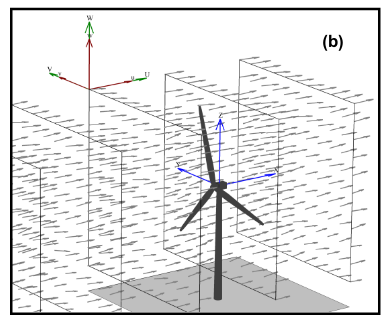
\includegraphics[width=0.5\textwidth]{./part1/figures/turbsim.png}
    \caption{Example of a turbulent wind field generated by TurbSim (source: \citealp{turbsim_2009}).}
    \label{fig:turbsim_simu}
\end{figure}

In their recent review of the challenges in wind energy, \citet{veers_2019_review} list some limits of the two spectral turbulence models recommended by the standards. 
First, their parameters were fitted using a restricted amount of data \citep{dimitrov_2017_turbulence_models_on_loads}. 
Second, the spatial coherence models associated with Kaimal models showed differences with turbulence measured on-site \citep{saranyasoontorn_2004}.  
Finally, recent studies showed that the choice of spectral model impacts the resulting wind turbine loads \citep{doubrawa_2019}. 
These approximations generally tend to overestimate wind flows, leading to conservative designs. 

To ensure more realistic turbulent wind field generation, two research perspectives are actively explored. 
Authors recently developed hybrid methods, including measurement data to enhance spectral models \citep{dimitrov_2017_constrained_turbulence}. 
Alternatively, higher fidelity models were studied in this domain, see for example the use of vortex methods \citep{branlard_2017_book} and large eddy simulations \citep{doubrawa_2019,bui_2022_mesoscale_LES}.  
Such complex models allow the simulation of mesoscale conditions (e.g., at the farm scale), and extreme transient events (e.g., gusts and storms). 
However, their computational cost is often prohibitive for UQ studies. 
When studying the wind resources at a wind farm scale, modeling wind energy losses induced by the turbines' wake becomes essential. 



%============================================================%
\subsection{Wake modeling}\label{sec:222}
%============================================================%

The wake is caused by the extraction of the wind kinetic energy, reducing the wind speed and increasing the turbulence downstream of the turbines (see the illustration in \fig{fig:wake_illustration}). 
In a wind farm, this effect depends on the spacing between turbines, as well as the ambient wind speed and turbulence intensity. 
The turbines positioned at the center of the farm are indeed the most impacted by the wake. 
As a wind farm owner, the consequence of the wake is twofold: a loss of energy production (in the range of 10 to 20 percent depending on the farm \citealp[Chap. 9]{burton_2021_wind_handbook}), and an increase in fatigue loads (due to the asymmetric loading added by the wake turbulences).

\begin{figure}%[h!]
    \centering
    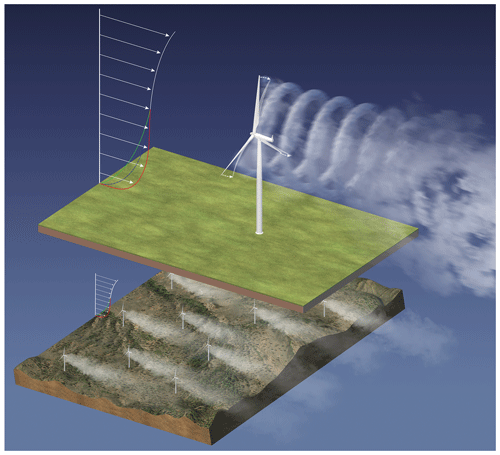
\includegraphics[width=0.5\textwidth]{./part1/figures/wake.png}
    \caption{Illustration of the wake created downstream a wind farm (source: \citealp{veers_2019_review}).} 
    \label{fig:wake_illustration}
\end{figure}

The initiation of the wake is a complex physical mechanism, however, the wake almost becomes axisymmetric after two turbine diameters downstream. 
At this stage, the wind speed deficit often presents a Gaussian profile centered on the hub \citep{burton_2021_wind_handbook}. 
Numerical models of different fidelities aim at simulating the wake. 
For example, computational fluid dynamics models give a detailed description of the wake but require high computational efforts. 
In practice, simple analytical models (often called ``engineering models'') are widely used and recommended by standards (see e.g., \citealp[Appendix E]{iec_2019}). 
These models mostly rely on the equivalence between the thrust load and the turbine wind energy deficit. 
Since the seminal engineering model proposed by \citet{jensen_1983_wake}, multiple enhancements were proposed. 
A wide benchmark of the wake modeling solutions for different fidelities was performed in \citet{doubrawa_2020_benchmark} and \citet{hiperwind_2023_wp3}. 
The optimal tuning of these engineering models was studied using measurements from a Doppler wind lidar in \citet{zhan_2020_optimal_wake}. 
Different software programs propose wake engineering models, such as FLORIS (developed by the NREL, see \citealp{fleming_2020_FLORIS}) and FarmShadow (developed by IFPEN\footnotemark). 

\footnotetext{FarmShadow: \url{https://www.ifpenergiesnouvelles.com/brief/wind-farm-optimization-wake-modeling-advances}}

To take into account the wake effect, control strategies increasingly move from the turbine scale to the farm scale. 
This concept, called ``active wake control'', introduces small yaw misalignments (making the control of turbines individually suboptimal) to optimize the global wake inside the farm \citep{rott_2018_active_control,simley_2020_active_control,meyers_2022_active_control}. 


%============================================================%
\subsection{Irregular wave generation}\label{sec:waves}
%============================================================%

The propagation of generated waves has been studied for a long time in hydrodynamics under the prism of different theories such as Airy's, and Stokes' ones \citep{goda_2010_waves}. 
Airy's wave theory (also referred to as the ``linear wave theory'') models sea states under the hypothesis of small waves relatively to the water depth.  
This spectral approach superposes many regular waves to model irregular waves. 
Two standard statistics are used in oceanography to represent sea states and their corresponding wave spectra: 
the wave period $T_p$ (with the corresponding frequency $f_p$), and the significant wave height $H_s$ (average over the highest third of the waves measured). 

The most commonly used parametric wave spectrum is named ``JONSWAP'', after the ``JOint North Sea WAve Project'' \citep{jonswap_1973} and is given by: 
\begin{equation}
    S(f) = \delta \frac{H_s^2}{f} \left(\frac{f_p}{f}\right)^4 \exp\left[-\frac54 \left(\frac{f_p}{f}\right)^4 \right] \gamma^\alpha,
    \label{eq:jonswap}
\end{equation}
where $f_p$ is the peak frequency, $\gamma^\alpha$ is a peak enhancement factor and $\delta$ is a weight coefficient (both defined in \citealp{milano_thesis_2021}). 
The JONSWAP spectrum is a corrected version of the Pierson-Moskowitz spectrum (proposed in \citealp{pierson_1964}), adding a peak enhancement factor $\gamma^\alpha$. 
Further details regarding the numerical values to choose in \eq{eq:jonswap} are given in \citet{burton_2021_wind_handbook}. 
An illustration of the two spectra is presented in \fig{fig:jonswap}, revealing the enhancement factor proposed in the JONSWAP model to better fit sea state measurements. 

\begin{figure}%[h!]
    \centering
    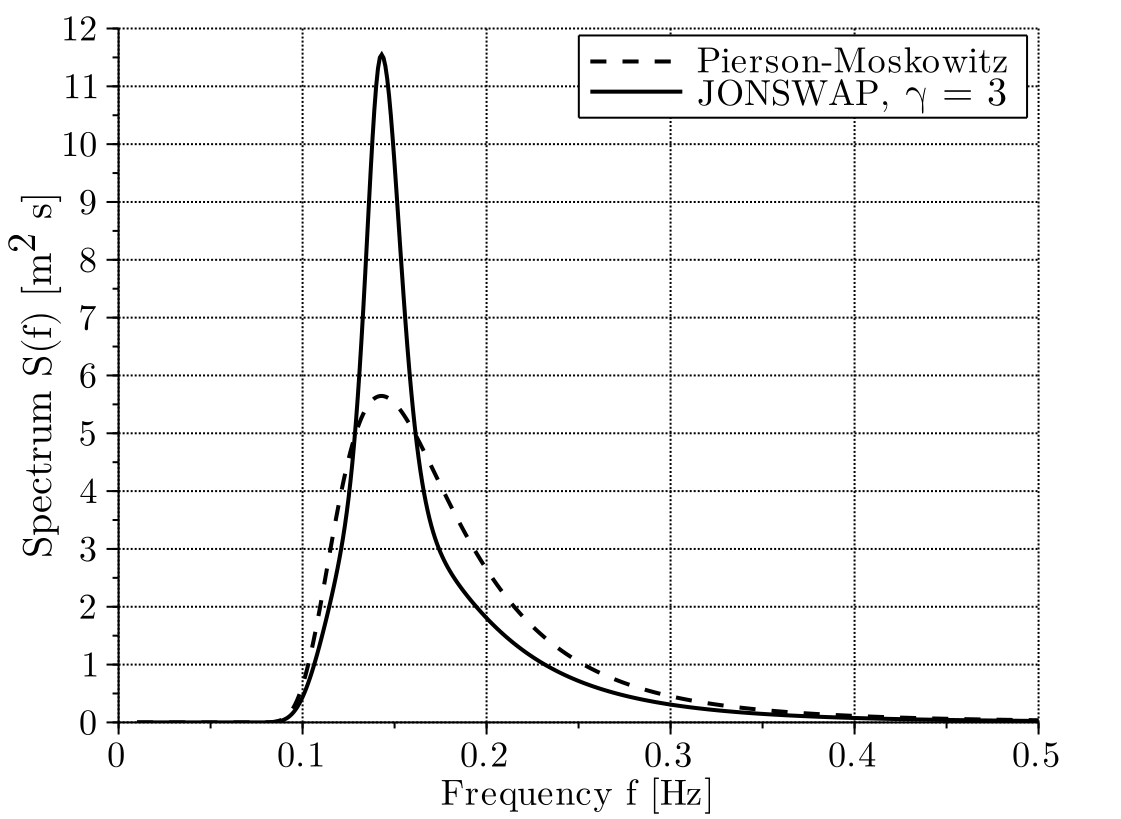
\includegraphics[width=0.45\textwidth]{./part1/figures/jonswap.png}
    \caption{Peirson-Moskowitz and JONSWAP spectra at significant wave height $H_s = 3$
    m and peak period $T_p = 7$ s (source: \citealp{milano_thesis_2021}).}
    \label{fig:jonswap}
\end{figure}

Swell waves are the result of weather conditions occurring far away from the location studied. 
Such waves usually present long wavelengths, allowing them to propagate over long distances with little dissipation. 
To take them into account, the unimodal wave spectrum introduced in \eq{eq:jonswap} was improved. 
Different methods allow building a parametric bimodal distribution, with a mode in the low frequencies corresponding to the swell. 
\citet{guedes_2005_bimodal_jonswap} reviews different bimodal wave spectra and compares their adequacy with measured sea states. 



%============================================================%
%============================================================%
\section{Wind turbine multi-physics modeling} \label{sec:owt_modeling}
%============================================================%
%============================================================%

OWT models are coupling several physics such as aerodynamics, hydrodynamics, mechanical elasticity, control, as well as mooring dynamics for floating OWT. 
Similarly to the usual practices from the offshore oil \& gas industry, OWT models were first built in the frequency domain. 
At an early design stage, a study in the frequency domain gives a rough idea of the system's feasibility by computing its natural frequencies. 
An OWT should not have its natural frequencies (or the blades and rotor frequencies, later introduced as 1P and 3P) in the same range as the main frequencies of the wave energy spectra. 
Otherwise, such systems can be subject to critical dynamic resonance, leading to their failure.

Beyond this preliminary check, frequency-domain approaches present limits for OWT modeling. 
As they rely on linear assumptions, they are unable to model the nonlinearities and transient loading phases \citep{matha_2011_ISOPE}. 
These aspects happen to be essential in the design of OWTs \citep{jonkman_2011_ISOPE}. 
As an alternative, the behavior of OWT systems is also simulated in the time domain. 

In the time domain, such systems may be modeled at different fidelity levels. 
The diagram in \fig{fig:owt_modeling_fidelities} illustrates the increasing complexities of two physics involved in OWT modeling, aerodynamics and structural dynamics respectively. 
Generally, the computational cost increases with the model fidelity, making UQ intractable at some point. 
In the present work, the numerical model of an OWT studied is actually a chain of three models executed sequentially (as illustrated in \fig{fig:owt_chained_model}): 
\begin{itemize}
    \item \textbf{TurbSim}: a turbulent wind generator (see Subection~\ref{sec:221});
    \item \textbf{\abv{diego}\footnotemark}: a multiphysics wind turbine model in the time domain (see Section~\ref{sec:owt_modeling}); 
    \item \textbf{Fatigue assessment}: a post-precessing computing fatigue damage (see Subsection~\ref{sec:235}). 
\end{itemize}
DIEGO is a numerical model developed by EDF R\&D to simulate the aero-hydro-servo-elastic behavior of OWTs in the time domain. 
Different extensive code-to-code comparisons between DIEGO and other aero-hydro-servo-elastic models showed close results. 
For instance considering bottom-fixed OWT \citep{popko_2021_DIEGO_benchmark} or floating OWT \citep{robertson_2020_diego_benchmark,kim_natarajan_2022}, DIEGO was compared to ``OpenFAST'' (developed by NREL), ``HAWC2'' (developed by DTU), ``BLADED'' (developed by DNV), and ``DeepLines Wind'' (developed by Principia). 

\footnotetext{DIEGO stands for ``Dynamique Int\'{e}gr\'{e}e des Éoliennes et G\'{e}n\'{e}ratrices Offshore''}

% Note that the wake should also be considered at the wind farm scale, as described earlier. 
\begin{figure}[h]
    \centering
    %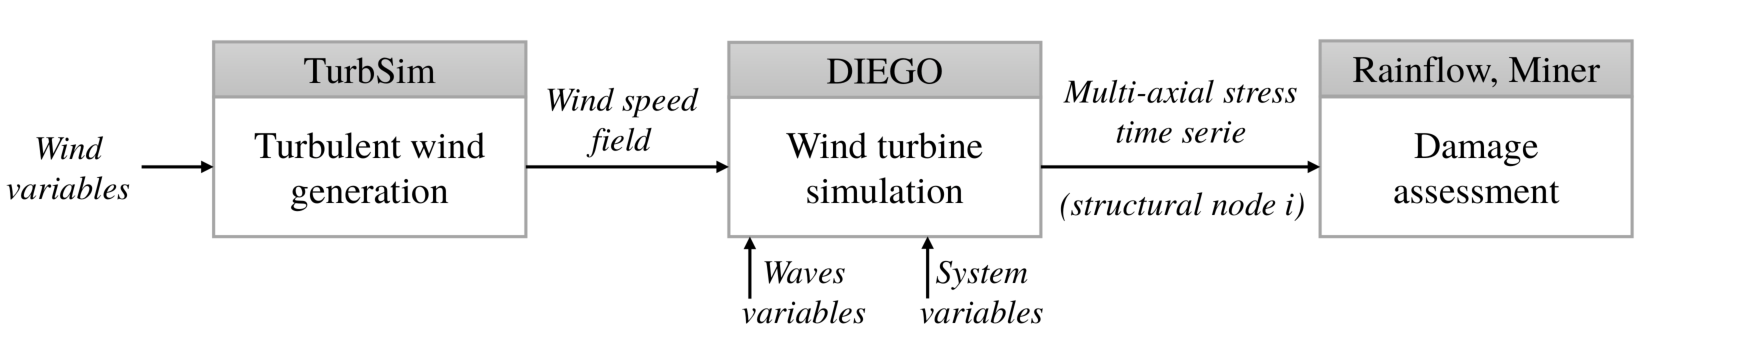
\includegraphics[width=0.8\textwidth]{./part1/figures/chained_model.pdf}
    \begin{tikzpicture}
    \node [style={grey_rect}] (0) at (0.5, 0) {Turbulent wind generation};
    \node [style={grey_rect}] (1) at (5, 0) {Wind turbine simulation};
    \node [style={grey_rect}] (2) at (9.5, 0) {Damage \\assessment};
    \node [style={grey_full_rect}] (3) at (0.5, 0.55) {TurbSim};
    \node [style={grey_full_rect}] (4) at (5, 0.55) {DIEGO};
    \node [style={grey_full_rect}] (5) at (9.5, 0.55) {Rainflow, Miner};

    \node [style=texte] (8) at (2.75, 0.3) {Wind speed\\field};
    \node [style=texte] (6) at (7.25, 0.1) {Multi-axial stress\\time series\\[3pt](structural node $i$)};
    \node [style=texte] (9) at (4.6, -1) {Wave\\variables};
    \node [style=texte] (10) at (6.2, -1) {System\\variables};
    \node (11) at (4.2, -1) {};
    \node (12) at (4.2, -0.4) {};
    \node (13) at (5.7, -1.) {};
    \node (14) at (5.7, -0.4) {};
    \draw [style=arrow] (13.center) to (14.center);
    \draw [style=arrow] (11.center) to (12.center);
    \draw [style=arrow] (1) to (2);
    \draw [style=arrow] (0) to (1);
\end{tikzpicture}
    \caption{Chained numerical model of offshore wind turbine.}
    \label{fig:owt_chained_model}
\end{figure}


\begin{figure}
    \centering
    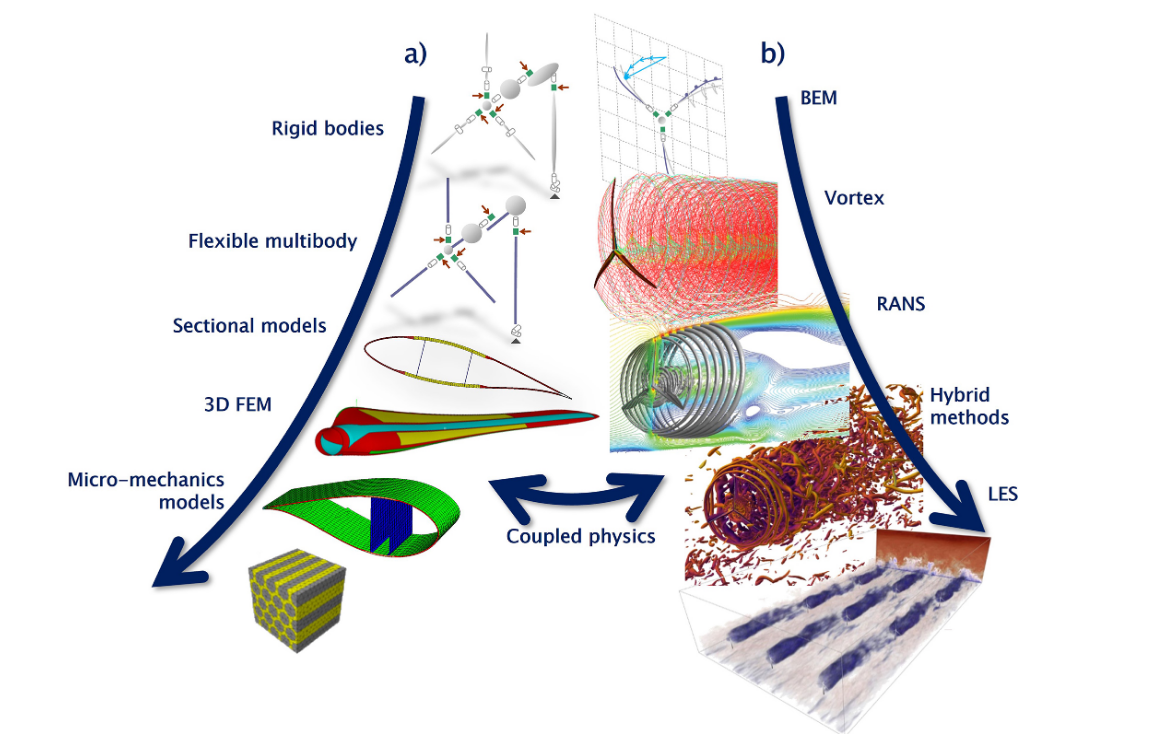
\includegraphics[width=0.7\textwidth]{./part1/figures/OWT_modeling_fidelities.png}
    \caption{Hierarchy of structural (a) and aerodynamic (b) wind energy systems models (source: \citealp{veers_2019_review}).}
    \label{fig:owt_modeling_fidelities}
\end{figure}



%============================================================%
\subsection{Aerodynamics of horizontal axis wind turbines}
%============================================================%

The blade ``element momentum theory'' (BEM in \fig{fig:owt_modeling_fidelities}) mixes different concepts to compute the aerodynamic forces on the rotating blades of the wind turbine. 
In this coupled physics model, aerodynamics affects the structural response and vice versa. 
To solve this problem, algorithms used in DIEGO first assess the apparent speed of elementary blades, to recover the lift and drag coefficients. 
The elementary loads are then integrated over each blade and communicated to the structural model.


\paragraph{Momentum theory.}
%------------------------------------------------------------%
At the core of wind turbine's aerodynamics, the concept of \textit{momentum theory} assumes that the air stream passing through the rotor disk is bounded by a stream tube of circular surface (not mixing with the ambient air). 
\fig{fig:actuator_disk} shows a longitudinal representation of the actuator disk and the way it affects the air upstream and downstream of the rotor. 
The associated momentum theory assumes the conservation of airflow at any cross-section (of area $A$) during a given time period. 
Passing through the actuator disk, the wind speed slows down and the static pressure drops which results in the wake. 
This pressure drop generates an axial force (called \textit{axial thrust force}) and a torque on the actuator disk.

\begin{figure}[!h]
    \centering
    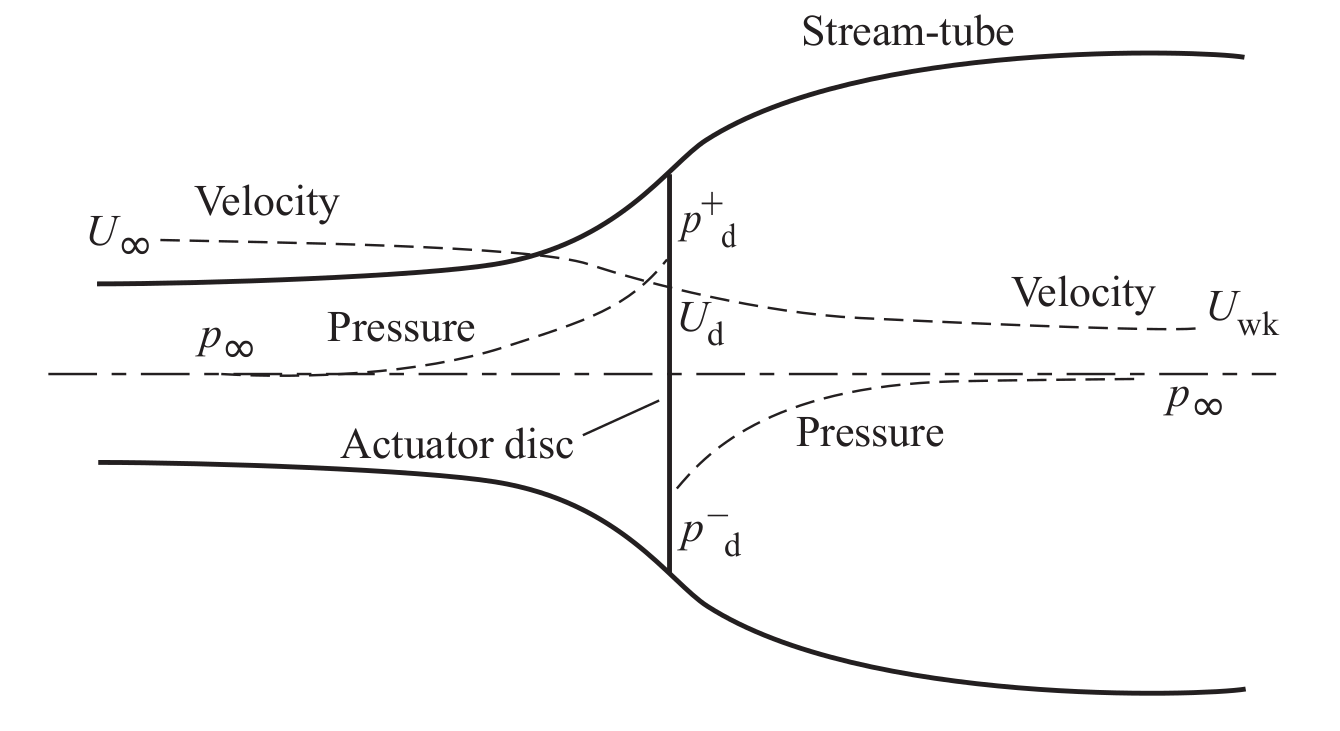
\includegraphics[width=0.6\textwidth]{./part1/figures/actuator_disk.png}
    \caption{Actuator disk model of the energy extraction (source: \citealp{burton_2021_wind_handbook}). Longitudinal evolution of the air pressure and wind speed along the wind stream.}
    \label{fig:actuator_disk}
\end{figure}
Considering the upstream flow, the flow at the rotor disk and the airflow in the wake, respectively denoted by the subscripts $\{\infty, d, \mathrm{wk}\}$, the following equality comes:  
\begin{equation}
    \rho A_\infty U_\infty = \rho A_d U_d = \rho A_{\mathrm{wk}} U_{\mathrm{wk}} \, ,
\end{equation}
where $U$ is the wind speed, $A$ the stream-tube area, and $\rho$ the air density. 
The wind speed in at the rotor disk can be expressed using the induction factor $\nu$ in the following expression: 
\begin{equation}
    U_d = U_\infty (1 - \nu), \qquad 0\leq \nu \leq 1.
\end{equation}
Using the momentum theory and Bernoulli's incompressible flow equation, one can express the aerodynamic thrust $T$ and power $P$ (see \citealp{milano_thesis_2021}) by: 
\begin{subequations}
    \begin{align}
        T&=(p_d^+ - p_d^-) A_d = 2 \rho A_d U_\infty^2 \nu (1- \nu),\\
        P&= T U_d = 2 \rho A_d U_\infty^3 \nu (1- \nu)^2.
    \end{align}
    \label{eq:momentum_theory}
\end{subequations}
The widely used power coefficient $C_P$ (respectively, thrust coefficient $C_T$) is the ratio of the power captured by the turbine against the total kinetic wind power available in the stream tube: 
\begin{subequations}
    \begin{align}
        C_P &= \frac{P}{\frac12 \rho A_d U_\infty^3} = 4\nu (1-\nu)^2,\\
        C_T &= \frac{T}{\frac12 \rho A_d U_\infty^2} = 4\nu (1-\nu). 
    \end{align}
\end{subequations} 
Betz's law is a theoretical limit value of the power coefficient $C_P^{\mathrm{Betz}} = 0.593$, obtained by canceling the power coefficient gradient \citep{burton_2021_wind_handbook}. 



\paragraph{Actuator disk.}
%------------------------------------------------------------%
Assuming a purely two-dimensional flow (meaning that the forces are only determined by the lift and drag coefficients), the blade element theory expresses the elementary thrust $\dd T$ and elementary torque $\dd Q$ applied on a blade element.

Considering the blade element represented in \fig{fig:blade_theory} at the blade length $r$, with airfoil chord $c$, angle of attack $\alpha$,  lift $C_L$ and drag $C_D$ coefficients, lift $L$ and drag $D$ forces, and the axial and tangential induction factors $a$ and $a'$. 
The axial thrust and torque exerted on a blade element are given by:
\begin{subequations}
    \begin{align}
        \dd T &= \frac12 \rho W^2 c \left(C_L \cos(\varphi) + C_D \cos(\varphi)\right) \dd r,\\
        \dd Q &= \frac12 \rho W^2 c \left(C_L \sin(\varphi) + C_D \sin(\varphi)\right) \dd r.
    \end{align}
    \label{eq:blade_element}    
\end{subequations}

\begin{figure}[h!]
    \begin{subfigure}[b]{0.5\textwidth}
        \centering
        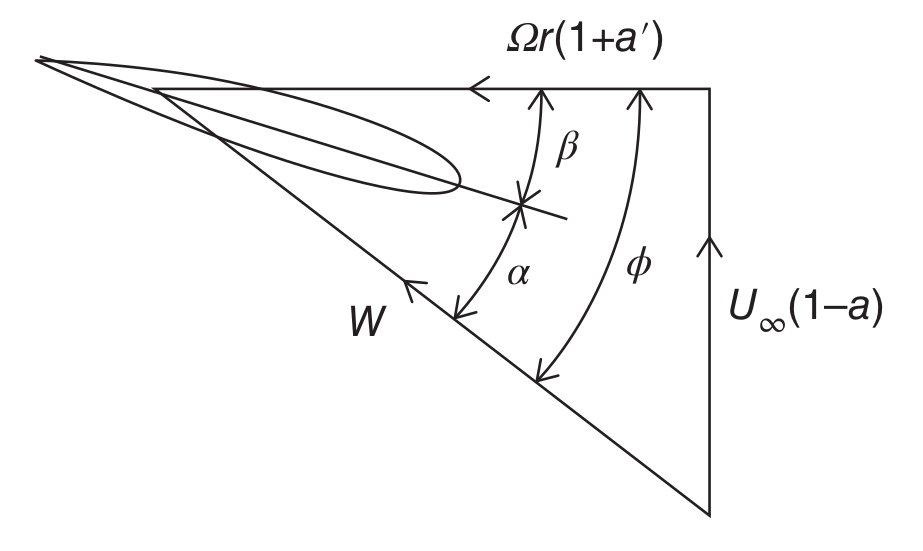
\includegraphics[width=0.9\linewidth]{./part1/figures/speed_triangle.png}
        \caption{Speed triangle.}
    \end{subfigure}
    \begin{subfigure}[b]{0.5\textwidth}
        \centering
        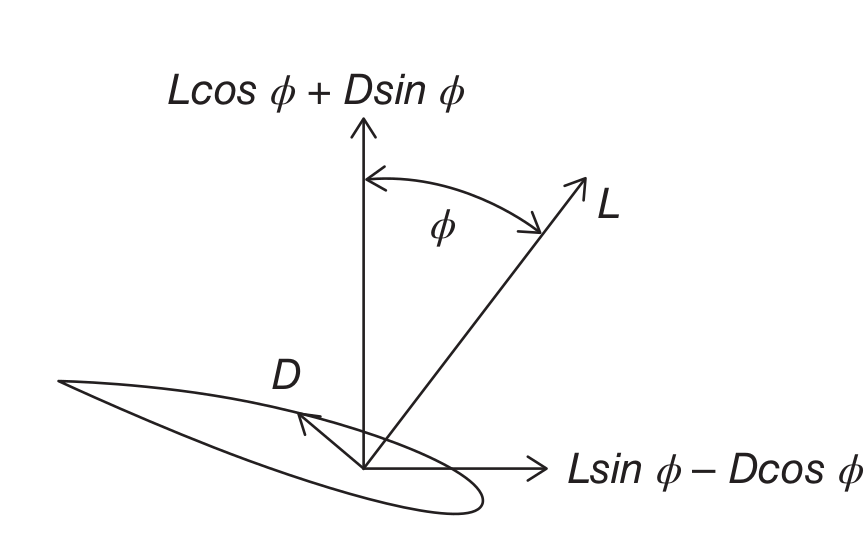
\includegraphics[width=0.9\linewidth]{./part1/figures/aerodyn_blade.png}
        \caption{Aerodynamic forces.}
    \end{subfigure}
    \caption{Blade element forces, with the lift and drag forces, $L$ and $D$ respectively, the flow angle $\phi$, the pitch angle $\beta$ and the angle of attack $\alpha$ (source: \citealp{burton_2021_wind_handbook}).}
    \label{fig:blade_theory}
\end{figure}
Finally, \textit{Blade element momentum theory} (\abv{bemt}) combines the results from blade element theory in \eq{eq:blade_element} with the results from momentum theory in \eq{eq:momentum_theory} to obtain the induction factors $a$ and $a'$. 
The resolution of this system of equations is often solved by iterative approaches (e.g., \citealp{dai_2011_BEMT}). 
Global axial thrust over the blade is then computed by integrating the elementary loads over all the elements. 
Note that various corrections are applied to the BEMT model, for example, to take into account the non-homogeneous loss of momentum over the rotor disk. 
The BEMT also fails to model nonlinear aerodynamic effects, for example, occurring with sudden changes in angle of attack, variation in wind velocity over the rotor disk, or yaw misalignment.
Such effects are sometimes called ``dynamic stall'' and are represented in DIEGO by the Beddoes-Leishman model (see \citealp{burton_2021_wind_handbook} for further details).  

%\elias{\paragraph{Aerodynamic damping?}}
%------------------------------------------------------------%
% See Petrovska p.51 


%============================================================%
\subsection{Hydrodynamics}
%============================================================%

As for hydrodynamic effects induced by waves, Morison's equations are a widely-used semi-empirical model to assess the hydrodynamic forces on thin fixed structures such as offshore oil platforms and wind turbines. 
Considering a slender cylindrical structure of diameter $D$, a flow velocity over time $u(t)$, the drag and inertial coefficients $C_d$ and $C_m$, the axial force $F$ (parallel to the flow direction) is given by:   
\begin{equation}
    F(t)\,=\,C_{m}\,\rho \,{\frac {\pi }{4}}D^{2}\,{\frac{\dd u(t)}{\dd t}}\,+\,C_{d}\,{\frac 12}\,\rho \,D\,u(t)\,|u(t)|.
\end{equation}
Standard values for the drag and inertial coefficients are often considered \citep{dnv_2013_offshore_design}. 
DIEGO uses Morison's equation together with a first-order potential solution to perform hydrodynamical simulations in the time domain.
An extended introduction to the hydrodynamics of fixed slender structures, as well as large floating structures, is given in \citep[Chap. 1]{milano_thesis_2021}.  

To design floating structures, more complex wave-loading models should be considered. 
For this purpose, \citet{ronge_2023_hydrodynamics_fowt} reviews nonlinear theories applied to the fluid-structure interactions of floating OWT and compares them to computational fluid dynamics results. 


%============================================================%
\subsection{Control}
%============================================================%
To maximize their energy production under turbulent wind conditions, wind turbines rely on their controllers. 
This aspect of wind turbines is usually kept confidential by manufacturers, as it gives them a competitive advantage.  
Indeed, the nacelle yaw angle should follow the wind direction to prevent any yaw misalignment (denoted by $\Theta_{\mathrm{yaw}}$). 
Nevertheless, the general control mode of a wind turbine depends on the wind speed. 
Two main ranges of operation are usually defined: first, between the cut-in and rated wind speed; second, between the rated and cut-off wind speed. 
These characteristic wind speed values are given by the turbine manufacturer. 
For example, a turbine may present a cut-in at $4~\mathrm{m.s^{-1}}$, a rated around $11~\mathrm{m.s^{-1}}$ and a cut-off at $25~\mathrm{m.s^{-1}}$. 
As a reminder, the wind turbine power $P$ derived from the momentum theory is such that: 
\begin{equation}
    P = \frac12 \rho \, A_d \, U_\infty^3 \, C_p(\beta,\lambda), 
    \label{eq:power_wt}
\end{equation}
where the power coefficient $C_p$ is a function of the pitch angle $\beta$ and the blade tip speed ratio $\lambda$, defined between the tangential speed on top of the blade and the wind speed: $\lambda = \frac{R \, \Omega}{U_\infty}$, for the rotation speed $\Omega$ and a rotor radius $R$. 

\paragraph{Below the rated wind speed.}
The goal of the control system is to extract as much power as available. 
A control strategy among the family of the \textit{maximum power point tracking} can be deployed \citep{abdullah_2012_control_review}.   
For example, the ``power signal feedback'' uses electromagnetic torque to control the power. 
This method first computes the maxima of the extracted power as a function of the rotation speed (using \eq{eq:power_wt}), for different speed values. 
Then, for a measured wind turbine rotation speed, the system can determine the reference maximal power. 
Considering this reference power, a controller (such as a proportional integral controller) intends to match the generated power with the reference by acting on the electromagnetic torque. 


\paragraph{Above the rated wind speed.}
The control system switches to a \textit{power limiting mode} by increasing the blades' pitch angles. 
By operating on the pitch, the rotation speed and the power produced are kept at their nominal values. 
This control is also often realized by a proportional integral controller \citep{bossanyi_2003_pitch_control}. 

A more exhaustive description of wind turbine control systems is available in \citet[Chap. 8]{burton_2021_wind_handbook}. 
More recent strategies often consider the control at the farm scale. 
As explained earlier, the operation of one turbine affects the others via the effect of its wake. 
Moreover, since wind energy production becomes significant in the electric mix, its production might be constrained to respect the stability of the grid (e.g., quality of the utility frequency).  
The work of \citet{gionfra_2018_control} studied optimal control strategies of wind farms considering the effects of the wake and the grid restrictions. 

%============================================================%
\subsection{Structural dynamics}
%============================================================%

The structural elements of modern wind turbines, such as the tower and the blades, compose a dynamic system subject to significant elastic deformations. 
Modeling an operating wind turbine therefore requires rigid body dynamics and linear elastic deformations. 
Altogether, various approaches were developed to model the structural dynamics of wind turbines: modal analysis, multibody methods and three-dimensional finite element methods. 
At the stage of preliminary designs, modal approaches can be used to represent the dynamics under linear assumptions \citep{hegseth_2019_modal_FOWT}. 
Then, the tower's natural frequencies assessed by a modal analysis can be compared with the wind, waves, and the rotor's frequencies. 
As illustrated in \fig{fig:modal_analysis}, the structure's natural frequency (denoted by $f_0$) should not coincide with the main excitation frequencies to avoid critical dynamic resonance.
In the case of a wind turbine, the rotor excitation creates a first dynamic load of frequency $f_{1P}$, while the three blades passing in front of the tower generate a second excitation of frequency $f_{3P}$.  
The \textit{soft-stiff} design strategy places the structure's natural frequency between the two rotor frequencies (i.e., $f_{1P} < f_0 < f_{3P}$ as described in \fig{fig:modal_analysis}) and avoids main frequencies of the wind and waves. 
For most floating designs the \textit{stiff-stiff} strategy is adopted, placing the natural frequency above the rotor frequencies (i.e., $< f_{3P}<f_0$). 

\begin{figure}
    \centering
    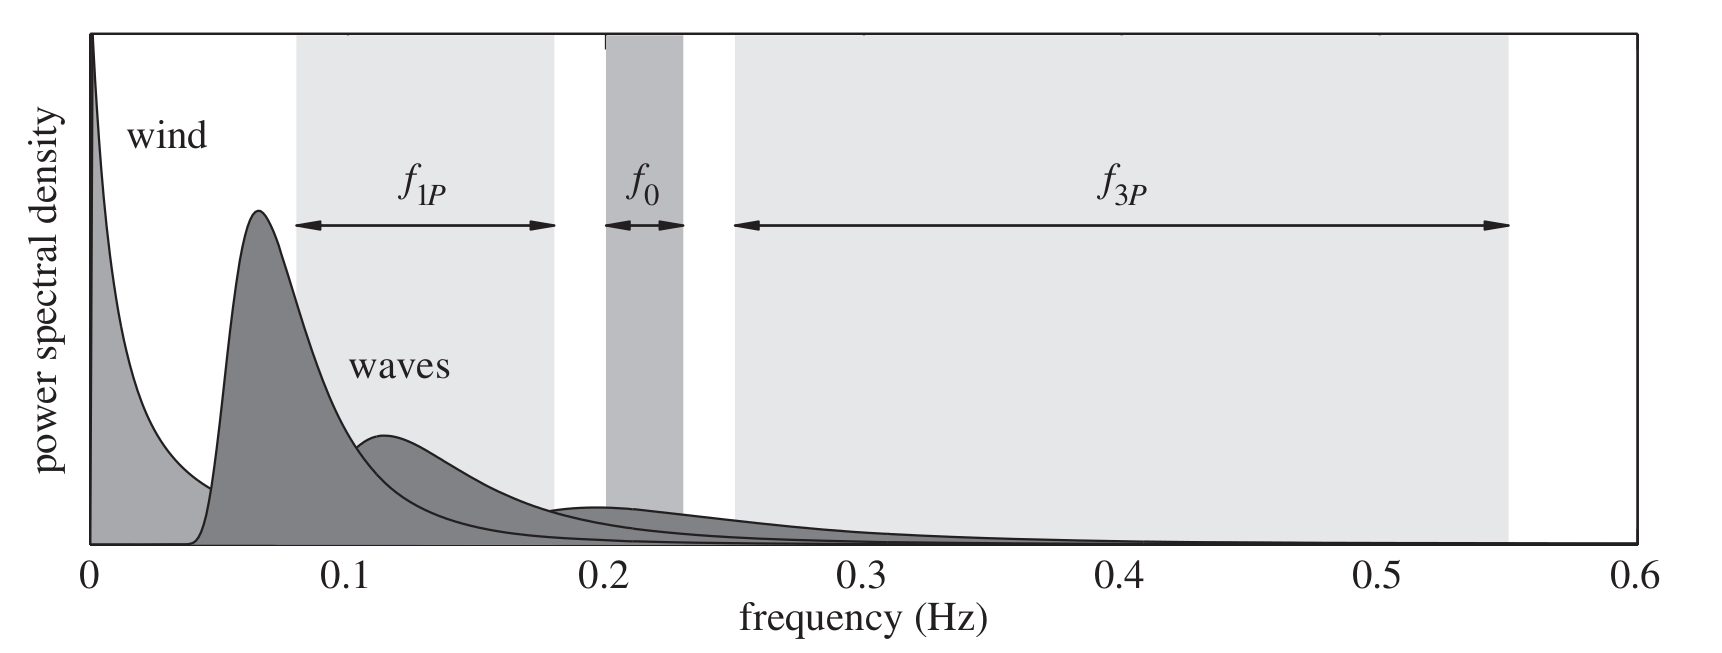
\includegraphics[width=0.75\textwidth]{./part1/figures/modal_analysis.png}
    \caption{Illustration of a soft-stiff design strategy, i.e., placing the structure's natural frequency $f_0$ away from the wind and wave power spectra, and the rotor excitation frequencies $f_{1P}$ and $f_{3P}$ (source: \citealp{kallehave_2015_modal}).}
    \label{fig:modal_analysis}
\end{figure}

However, modal analysis cannot be used to model transient loading phases and their corresponding nonlinearities, which is crucial beyond early design. 
For a higher fidelity, simulations in the time domain using flexible multibody approaches are commonly used to describe the nonlinear dynamics \citep{holm_2009_multibody,alsolihat_2018_flexible_multibody}. 
DIEGO implements such an approach by combining rigid multibody dynamics with a deflection model based on Lagrangian equations \citep{milano_thesis_2021}. 
Note that for the modeling of floating wind turbines, a preliminary step of rigid body dynamics is added to define the coordinate system of the floater. 
\citet{otter_2022_owt_modeling_review} reviews the state-of-the-art numerical and experimental modeling techniques for multi-physics OWT systems. 


%============================================================%
\subsection{Fatigue damage}\label{sec:235}
%============================================================%

Mechanical fatigue damage is a significant phenomenon to consider when designing wind turbines. 
It refers to the progressive weakening of a material subject to cyclic or repeated loading, which may be significantly lower than the material's ultimate strength. 
Understanding the mechanisms behind mechanical fatigue damage is essential for designing durable and reliable structures. 
To quantify the fatigue damage on OWT structures, standards \citep{dnv_fatigue_2016} recommend simulating the stresses in the time domain and identifying a series of stress cycles. 
Then, the so-called ``\abv{sn} curve'' (for ``stress-number of cycles'') of a specific material gives the number of cycles before failure at a given constant stress amplitude. 
After identifying the stress cycles identified on the results of the OWT simulation, an aggregation method (in our case, \textit{Miner's rule}) gathers the elementary damages over the stress time series studied. 


\paragraph{Stress cycle identification.}
%------------------------------------------------------------%
Offshore wind turbine simulators as DIEGO, deliver a time-dependent stress tensor. 
Although damage studies are commonly realized on the axial stress $\sigma_{11}$, the other components of the tensor could also be taken into account. 
To ease the manipulation of this tensor, the equivalent Von Mises stress is computed, turning a multiaxial stress into an equivalent uniaxial stress. 
One can also consider a ``plane strain'' hypothesis on the Cauchy stress tensor $\underline{\underline{\sigma}}$, which is expressed as:
\begin{equation}
    \underline{\underline{\sigma}} = \begin{pmatrix}
                            \sigma_{11} & \sigma_{12} & 0\\
                            \sigma_{21} & \sigma_{22} & 0\\
                            0 & 0 & \sigma_{33}
                            \end{pmatrix}.
\end{equation}
This assumption simplifies the expression of the equivalent Von Mises stress $\sigma_{\mathrm{VM}}$, given by: 
\begin{equation}
    \sigma_{\mathrm{VM}}=\sqrt{{\frac {1}{2}}\left[(\sigma _{11}-\sigma _{22})^{2}+(\sigma _{22}-\sigma _{33})^{2}+(\sigma _{33}-\sigma _{11})^{2}\right] + 3 \sigma _{12}^{2}}.
\end{equation}
Stress cycles can now be identified on the axial stress $\sigma_{11}$ or the equivalent Von Mises stress $\sigma_{\mathrm{VM}}$ time series. 
The usual method to identify fatigue stress cycles is called \textit{rainflow counting} \citep{dowling_1972}. 
In this approach, fatigue stress cycles are only defined by their amplitude (also called ``range'') and mean value, regardless of their chronology. 
Rainflow counting returns a list of stress ranges identified and denoted by $s \in \R_+$ in the following. 


\paragraph{S-N curve.}
%------------------------------------------------------------%
The S-N curve is also called the ``W\"ohler curve'' after the pioneer work of August W\"ohler. %, who demonstrated that fatigue damage was at the origin of railway accidents in the mid-19\textsuperscript{th} century \citep{schutz_1996_history_fatigue}. 
As a result of repeated fatigue experiments, this tool determines the number of similar stress cycles necessary to reach a fatigue ruin for a defined stress cycle amplitude. 
Its values depend on the material studied and on external conditions (in the offshore industry, various S-N curves distinguish the case in the air, underwater, with cathodic protection, etc.). 

A well-admitted simplification of the S-N curve is to consider it as log-linear\footnotemark~on two segments:
\begin{equation}
\log(N_{\mathrm{c}}(s)) = \left\{
    \begin{array}{ll}
        \log(a_1) - m_1 \log(s), & \mbox{for}~ s \in [s_{\mathrm{min}}, s_{\mathrm{e}}] \\
        \log(a_2) - m_2 \log(s), & \mbox{for}~ s \in [s_{\mathrm{e}}, s_{\mathrm{max}}]\, ,
    \end{array}
\right.
\end{equation}
where $N_{\mathrm{c}}$ is the predicted number of cycles to failure for stress range $s$, $m$ is the negative inverse slope of the S-N curve, 
$\log(a)$ is the intercept of log N-axis by the S-N curve, $s_{\mathrm{min}}$ is the minimal (resp. maximal) stress range identified by the rainflow counting, 
and $s_{\mathrm{e}}$ is the stress range axis of the intersection of the two log-lines formed by the S-N curve (see e.g., \fig{fig:probabilistic_SN}). 

\footnotetext{The logarithm related to the S-N curves in this document is in base 10.}

The expression of this curve in two linear segments arises from the concept of endurance limit of a material, denoted by $s_{\mathrm{e}}$, under which the effect of fatigue on a material should be considerably smaller. 
According to \cite{dnv_fatigue_2016}, the S-N curve is altered for welded tubular joints by taking into account the tube's thickness:
\begin{equation}
N_{\mathrm{c}}(s) = \left\{
    \begin{array}{ll}
        a_{1} \left(s \left(\frac{t}{t_{\mathrm{ref}}}\right)^h\right) ^{-m_1}, & \mbox{for}~ s \in [s_{\mathrm{min}}, s_{\mathrm{e}}]\\
        a_{2} \left(s \left(\frac{t}{t_{\mathrm{ref}}}\right)^h\right)^{-m_2}, & \mbox{for}~ s \in [s_{\mathrm{e}}, s_{\mathrm{max}}]
    \end{array}
\right.
\end{equation}
With $t_{\mathrm{ref}}$ the reference thickness (for tubular welded joints $t_{\mathrm{ref}}$ = 25 mm); $t$ the plate thickness, and $h$ the thickness exponent. 
The numerical values considered in the present work derive from the standards \citet[Sec. 2.4.6]{dnv_fatigue_2016}, and are reproduced in Table \ref*{tab:sn_table}. 

\begin{table*}[h]
    \centering
    \caption{S-N curve numerical values of welded tubular joints in different environmental conditions (source: \citealp{dnv_fatigue_2016}).}
    \begin{tabular}{l|l|l|l|l|l}
     \hline
     \textit{Environment} & $m_1$ & $log(a_1)$ & $m_2$ & $log(a_2)$ & $h$\\
     \hline
     Air & $3.0$ & $12.48$ & $5.0$ & $16.13$ & $0.25$\\
     Seawater with cathodic protection & $3.0$ & $12.18$ & $5.0$ & $16.13$ & $0.25$\\ Seawater free corrosion & $3.0$ & $12.03$ & $3.0$ & $12.03$ & $0.25$\\ 
    \end{tabular}
    \label{tab:sn_table}
\end{table*}

\paragraph{Nonzero mean correction.}
%------------------------------------------------------------%
Most S-N curves are built over zero mean stress cycles, however, other empirical models were developed to consider various stress mean $s_m$ \citep{suresh_1998_fatigue_book}. 
Therefore, the S-N curve becomes a three-dimensional envelope depending on the number of cycles $N_c$, the stress amplitude $s$, and the mean stress $s_m$. 
The ``Goodman line'' and the ``Gerber parabola'' are two models relating the stress amplitude $s$ to the mean stress $s_m$:  
\begin{align}
    \mathrm{Goodman} &:\quad \frac{s}{s_e} + \frac{s_m}{R_m} = 1\, ,\\
    \mathrm{Gerber} &:\quad \frac{s}{s_e} + \left(\frac{s_m}{R_m}\right)^2 = 1\, ,
\end{align}
where the material's yield stress is denoted by $R_m$ and the endurance limit by $s_e$. 
The Haigh diagram represented in \fig{fig:haigh_diagram} is a slice of the three-dimensional envelope for fixed values of fatigue endurance (i.e., number of cycles). 
By comparing the two models visually, the Goodman line (which is the most used in the literature) is the most conservative. 
Further discussion in the field of wind turbines was proposed in the early 2000s with a focus on the fatigue endurance of glass fiber materials \citep{sutherland_2000_fatigueWT}. 
In the present work, the nonzero correction presented above is not considered as the values of mean stress were found to be negligible compared to the yield stress of the steel material studied. 

\begin{figure}
    \centering
    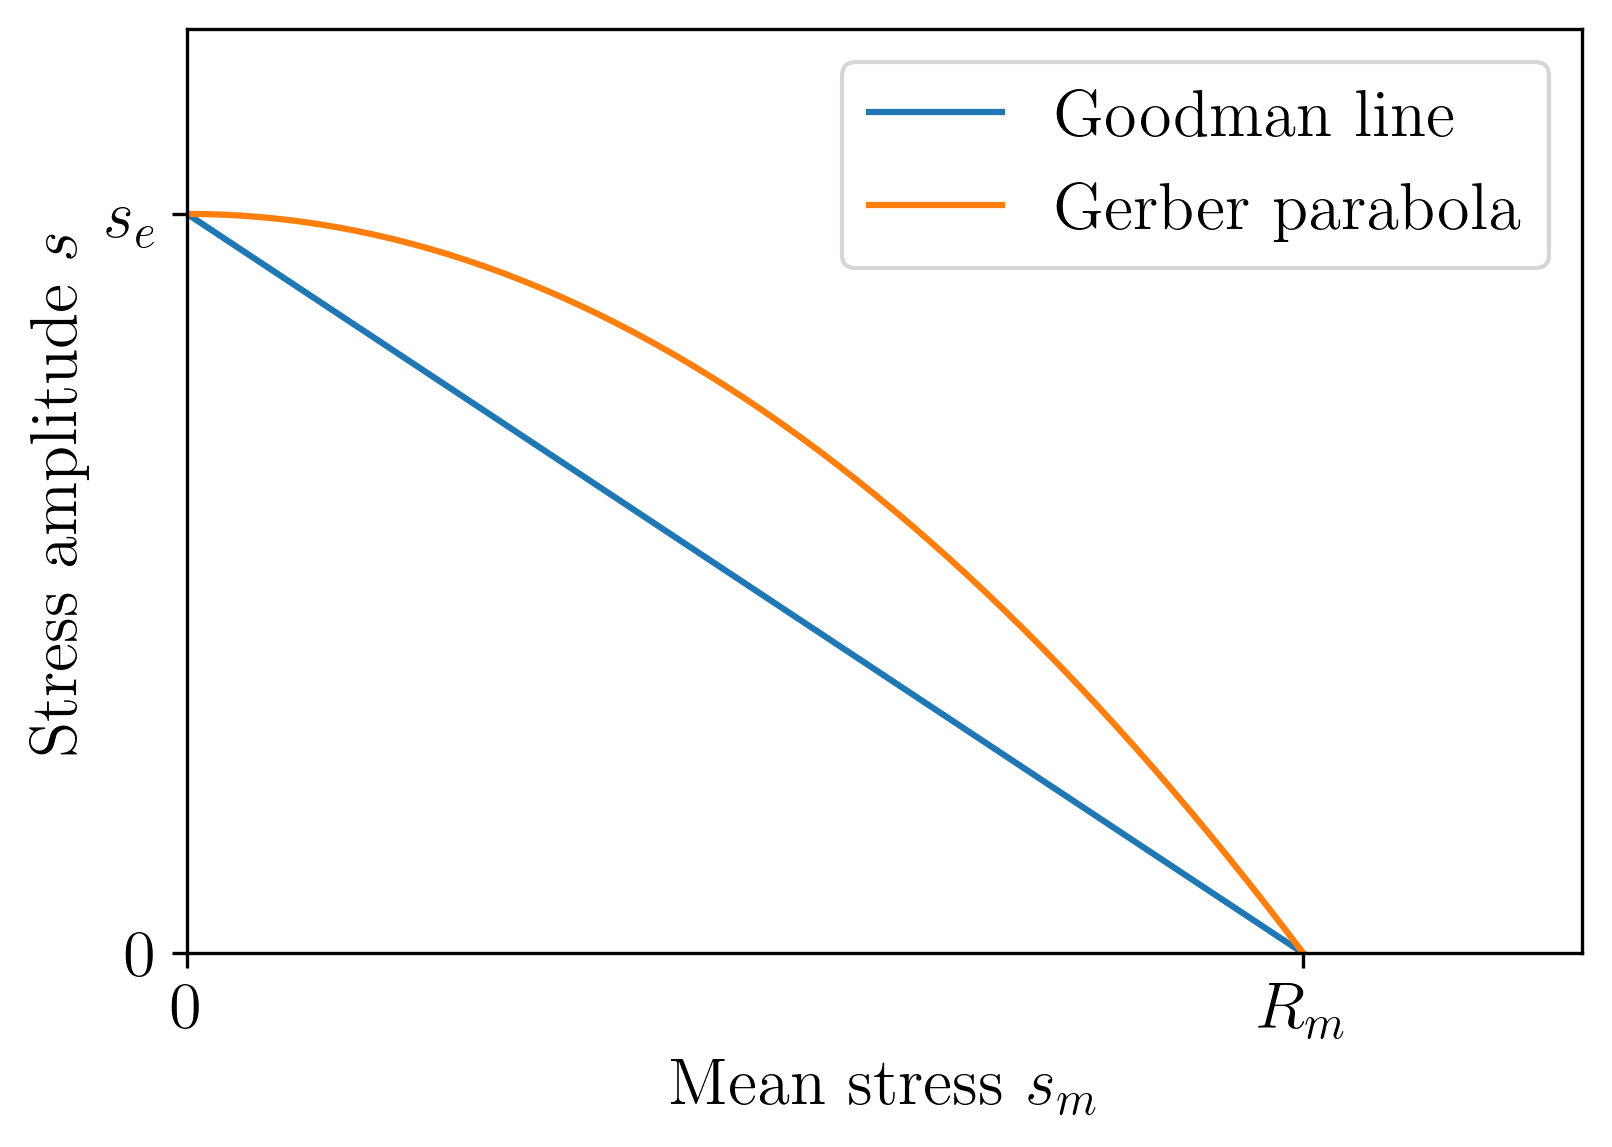
\includegraphics[width=0.5\textwidth]{../numerical_experiments/chapter2/figures/haigh_diagram.png}
    \caption{Illustration of the Haigh diagram representing the combination of mean stress and amplitude leading to the same fatigue endurance.}
    \label{fig:haigh_diagram}
\end{figure}



\paragraph{Cumulative damage theory.}
%------------------------------------------------------------%
A popular approach to assess the damage cumulated on a stress time series is to consider the fatigue contribution of each stress cycle according to the S-N curve. 
Palmgren-Miner's rule defines the \textit{cumulative damage} $d_{\mathrm{c}}$ by summing the fatigue contributions of each stress cycle $j, j \in \{1, \dots, k\}$, regardless of their order of appearance:
\begin{equation}
    d_{\mathrm{c}} = \sum_{j=1}^{k} \frac{1}{N_{\mathrm{c}}\left(s^{(j)}\right)} \, .
    \label{eq:miner}
\end{equation}
In this theory, the material reaches fatigue ruin when $d_{\mathrm{c}} \geq 1$.  
A common practice when using Palmgren-Miner's rule is to gather the stress cycles in a set of bins. 
This practice induces an integration error, which becomes significant as the number of bins is reduced. 
In the following, the cumulative damage is computed without binning, as defined in \eq{eq:miner}.

Spectral methods were also introduced to quantify fatigue damage in the late 1980s. 
The main idea is to infer a PDF over the amplitudes of the stress cycles identified by rainflow counting, typically using a mixture of parametric distributions. 
From this PDF, one can derive the fatigue endurance and the cumulated damage (see further details in the review of \citealp{dirlik_2021}). 
Spectral approaches showed to be well suited at early design phases but not ideal for some tasks (e.g., for blades' fatigue \citealp{ragan_2007_dirlik_vs_miner}). 
%Overall, fatigue estimation in the time domain does not represent a large computational effort compared to the simulation of the wind turbine's physics. 

Finally, nonlinear fatigue models were developed in the 1990s \citep{fatemi_1998} to take into account the order in which the loading cycles were applied to the structure. 
For OWT applications, the recent work of \citet{rocher_2020_nonlinear_fatigue} studied a probabilistic version of nonlinear fatigue models. 
Unfortunately, this refined approach requires a larger computational effort and a calibration step over experimental tests of various parameters \citep{freyssinet_2023_nonlinear_fatigue}.  


%============================================================%
%============================================================%
\section{Design and operation practices} \label{sec:owt_design}
%============================================================%
%============================================================%

The design and operation of OWT are at the intersection of various engineering, environmental and social considerations. 
Regardless of the different bottom-fixed or floating technologies, OWTs are dynamically excited structures evolving in a harsh offshore environment.   
To operate such assets over up to 25 years of lifespan, multiple aspects should be assessed, from soil modeling, studies of environmental impact, grid integration, manufacturing quality, port logistics, to marine growth management, and maintenance. 
This section resumes the main types of OWT technologies, as well as the main design and operation practices.   

%============================================================%
\subsection{Types of technologies and preliminary design}
%============================================================%
The multiple OWTs technologies developed over the last two decades can be gathered into two groups: bottom-fixed or floating technologies \citep{eolien_en_mer_2022}. 
\fig{fig:FOWT_bottomfixed} and \ref{fig:FOWT_floating} respectively illustrate the different types of bottom-fixed or floating technologies. 
At this stage, the bottom-fixed solutions present more maturity while floating technologies are still transitioning from the phase of large demonstrators to industrial wind farms. 
In France, the current development of offshore wind energy has led to the construction of the two first industrial projects (both managed by EDF Renewables). 
On the coast of Saint-Nazaire, 80 bottom-fixed wind turbines were built on monopile foundations, with a total power of 480 MW. 
On the Mediterranean coast, the first French industrial floating project was recently installed 20 km offshore from the coast of Fos-sur-Mer near Marseille. 
This pilot project called ``\textit{Provence grand large}'', is composed of three turbines operating on so-called ``tension-leg platforms'', delivering 25 MW of nominal power.     

In order to lift water depth limitations associated with bottom fixed technologies (technical limit around 60 meters), floating pilot projects have emerged across the world. 
However, the wind energy industry still tests different floating technologies in terms of cost efficiency and durability (as listed in \citealp{mackinnon_2022_FOWT_table}). 
An example of some farm projects with different types of technologies is described hereafter: 
\begin{itemize}
    \item \textbf{Semi-submersible}: a pilot project of three 10 MW turbines called ``\textit{les \'{e}oliennes du Golfe du Lion}'' in the south of France relies on a semi-submersible technology developed by the company Principle Power \citep{cermelli_2018_windfloat};   
    \item \textbf{Tension-leg}: a pilot project of three 8 MW turbines called ``\textit{Provence grand large}'' exploits tension-leg platforms co-developed between the IFPEN national laboratory and the company SBM \citep{caille_2017_TPL_IFPEN}; 
    \item \textbf{Barge}: a pilot project of three 10 MW turbines called ``EOLMED'' uses the floater developed by the company Ideol \citep{guignier_2016_ideol}; 
    \item \textbf{Spar}: the Norwegian oil and gas company Equinor chose the ``spar'' technology (see \fig{fig:FOWT_floating} and \citealp{driscoll_2016_hywind}) to equip its floating wind farm of 88 MW, named ``Hywind Tampen''. 
\end{itemize}

\begin{figure}
    \begin{subfigure}[b]{0.48\textwidth}
        \centering
        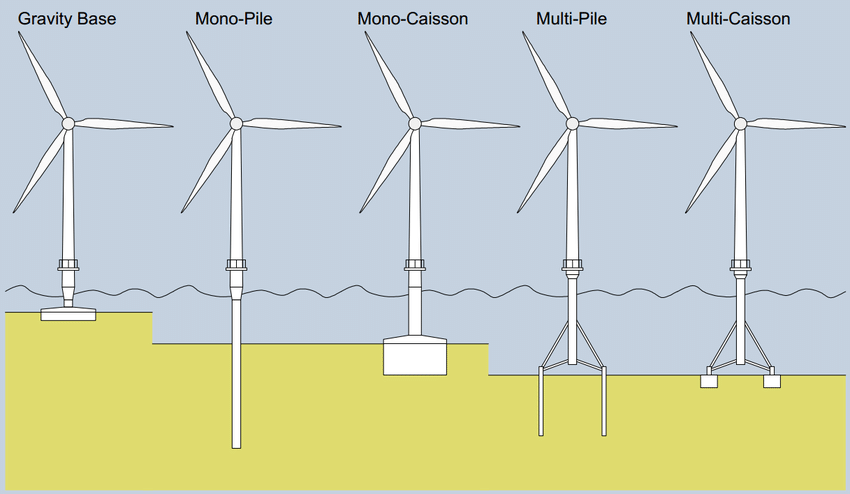
\includegraphics[width=\linewidth]{./part1/figures/bottom_fixed_techno.png}
        \caption{Bottom-fixed.}
        \label{fig:FOWT_bottomfixed}
    \end{subfigure}
    \begin{subfigure}[b]{0.48\textwidth}
        \centering
        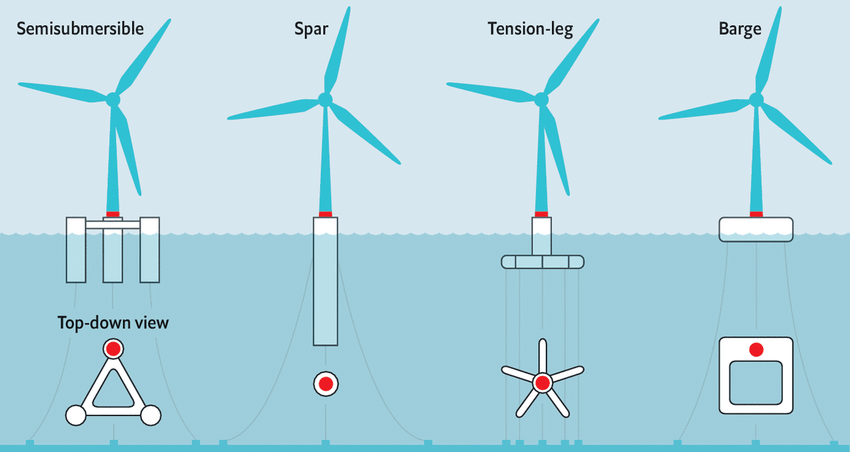
\includegraphics[width=\linewidth]{./part1/figures/Floating-wind-platform-categories.png}
        \caption{Floating.}
        \label{fig:FOWT_floating}
    \end{subfigure}
    \caption{Main bottom-fixed (left) and floating (right) OWT technologies (sources: \citealp{ahmed_2015_bottomfixed_image,mei_2021_FOWT_illustration}).}
\end{figure}

The turbines installed offshore over bottom-fixed foundations or floating structures present the same properties and components. 
As described in \fig{fig:owt_diagram}, the structure of a wind turbine is composed of blades made of composite materials, while the tower, the transition piece and the foundation (e.g., monopile) are made out of steel. 
The type of steel used for the foundation and the tower are typical structural steel (i.e., steel with low carbon concentration such as the S355). 

Inside the nacelle, the gearbox adapts the rotation speed to suit the energy conversion system (i.e., the generator). 
Manufacturers also develop solutions without gearbox, called ``direct-drive'', to improve the components' reliability. 
This technology is relevant offshore, as the maintenance constraints are more drastic. 
However, the corresponding generators used in this situation operate at a lower rotation speed. 
Adapting the generators to this speed range significantly increases their weight and requires the use of larger permanent magnets, thus increasing the whole price.   

The construction of an offshore wind farm requires several years of project planning, administrative procedures, consultation with public opinion, and design. 
International standards define the recommended practices and requirements related to the design and operation of OWTs. 
Among them, the IEC 61400 is subdivided into many parts, including the general one \citep{iec_2019} and other parts detailing specific topics.       
To validate the structural integrity of a wind turbine design, the standards recommend simulating the behavior of the OWT (using the methods described in Section~\ref{sec:owt_modeling}) for many environmental conditions, called ``design load cases'' (DLCs). 
As the environmental conditions depend on the site studied, the standards provide generic DLCs depending on a rough classification of the environmental conditions. 
Following the terminology in civil engineering, the structure is mainly designed for ``fatigue limit states'' (\abv{fls}) and ``ultimate limit states'' (\abv{uls}) w.r.t. environmental conditions. 
For fatigue, advanced sampling methods relying on environmental data measured on-site will be introduced in Chapter~\ref{chpt:4}. 
Beyond the main solicitations resulting from environmental loading, various aspects should be considered around OWTs. 

\begin{figure}
    \centering
    \begin{subfigure}[b]{0.3\textwidth}
        \centering
        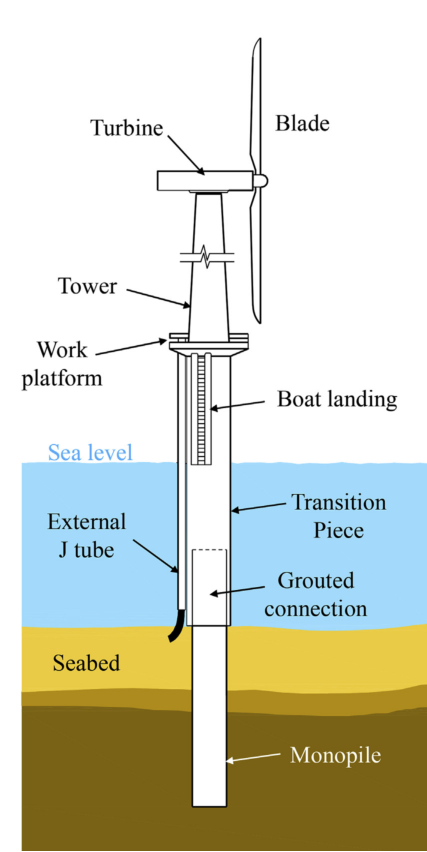
\includegraphics[width=0.7\linewidth]{./part1/figures/owt_diagram.pdf}
        \label{fig:struc_components}
        \caption{Monopile structure diagram.}
    \end{subfigure}
    \begin{subfigure}[b]{0.48\textwidth}
        \centering
        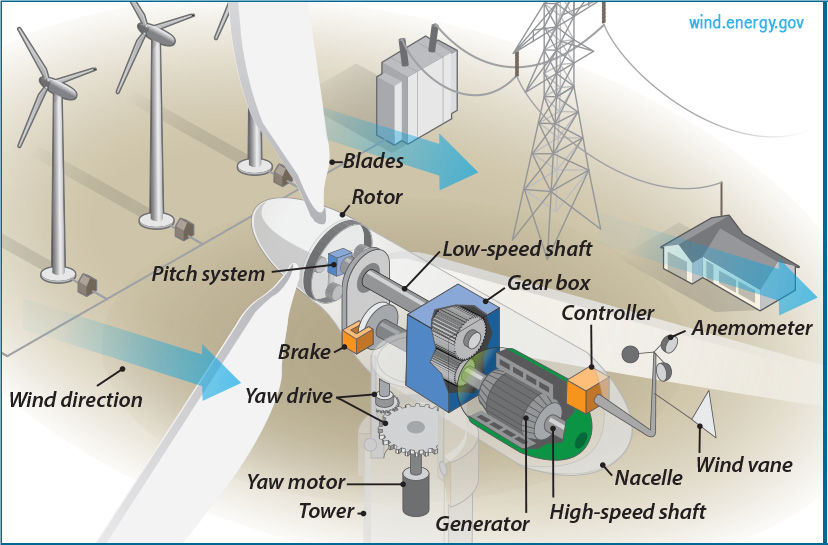
\includegraphics[width=\linewidth]{./part1/figures/nacelle_components.png}
        \caption{Major components in the nacelle.}
        \label{fig:nacelle_components}
    \end{subfigure}
    \caption{Diagrams of an OWT structure (source: \citealp{chen_2018_owt_diagram}) and nacelle (source: U.S. Department of Energy).}
    \label{fig:owt_diagram}
\end{figure}

%============================================================%
\subsection{Further design considerations}
%============================================================%
The present section focuses on different topics to be addressed ahead of, or during the design and operation of OWTs.

\paragraph{Soil modeling.}
%------------------------------------------------------------%
The accurate geotechnical description of an offshore site plays an important role in the design and stability of bottom-fixed OWTs. 
The seabed soil properties are far from uniform in a wind farm, forcing the designer to adapt the foundations within a farm. 
Prior to the installation, geotechnical surveys and soil testing are conducted to assess parameters such as soil composition, density, strength, and seabed stability. 

To model the dynamic behavior of foundations, certification companies adapted their methods from the oil and gas industry to offshore wind energy \citep{dnv_2018_soil}. 
For monopile foundations, the ``$p-y$'' method is often used to model soil-structure interactions. 
Assuming that these interactions are purely lateral, this method defines a set of nonlinear lateral springs along the foundation's height.  
Together, the springs model the relation between the soil resistance ``$p$'' and the lateral displacement ``$y$''. 
Generally speaking, monopile foundations for OWT tend to be more rigid than the piles for oil and gas platforms, as the cyclic loading on wind turbines induces more fatigue (see the case study presented in \citealp{le_2014_geotech_casestudy}).  
However, various contributions in wind energy extended the use of $p-y$ curves to the case of multidirectional and irreversible displacements \citep{lovera_2019_thesis}. 
In summary, geotechnical considerations are essential for offshore wind turbine design, and the variability of soil properties within a wind farm necessitates a tailored approach to foundation design. 
Finally, the consideration of uncertainties in this field is still an open research topic \citep{reale_2021_OWT_soil_uncertainties}.

%\elias{Describe the modeling method in DIEGO called the ``apparent fixity'', and the defined soil stiffness matrix. See Petrovska p.52.}


\paragraph{Marine growth.}
%------------------------------------------------------------%
The bio-colonization of offshore structures and submarine cables is a significant concern in the maintenance and operation of OWTs. 
Elements exposed to the colonization of marine organisms, such as mussels, can cause several adverse effects. 
Firstly, the added weight increases the mass of the turbine and its foundation, potentially changing the dynamics of the systems and its structural integrity \citep{ameryoun_2019_marine_growth,schoefs_2022_reliability_marine_growth}. 
Secondly, marine growth changes the surface's roughness of the submerged components, which can create fluctuating hydrodynamic loads and vibrations \citep{marty_2021_cable_marine_growth}. 
To limit its impact on the reliability of OWTs, this phenomenon is addressed with regular preventive cleaning measures as part of the maintenance planning. 


\paragraph{Global scour.}
%------------------------------------------------------------%
The large-scale erosion of seabed sediment around bottom-fixed offshore wind turbine foundations also called ``scour'', raises different problems. 
As global scour is a critical element of the long-term OWT reliability, various mitigation measures are reviewed in \citet{fazeres_2021_scour}, including scour protection, and scour-robust foundation design.
When scouring occurs, the stability of the foundation is first reduced, potentially leading to tilting. 
Moreover, the load distribution changes, causing uneven stresses and increased fatigue. 
Finally, submarine cable exposure increases the risk of damage and electrical faults. 


\paragraph{Port logistics.}
%------------------------------------------------------------%
In the installation and maintenance of such large-scale systems, port logistics plays a key role considering the international supply chain involved. 
The coordination, transportation and assembly of massive wind turbine components, foundations, and supporting infrastructure requires meticulous planning and execution. 
In accordance, the costs of handling operations and maintenance represent a large share of the \textit{levelized cost of energy} \citep{shields_2021_owt_lcoe}.  

In his review of OWT installation techniques, \citet{jiang_2021_owt_installation_review} describes the foundations' and components' installation processes depending on the OWT technology. 
Because of their large scale, most structural assembly (e.g., blades, or floater) are done on dedicated port docks, making the port choice critical.  
The assembled turbines are then transferred offshore with specialized vessels, such as installation jack-ups. 
Timing and synchronization are critical, as weather windows for handling operations can be limited.


\paragraph{Grid integration.}
%------------------------------------------------------------%
Unlike traditional centralized energy production plants (i.e., nuclear and fossil), wind energy has a considerable impact on grid management. 
The intermittency of offshore wind generation is driven by variable wind conditions, which disrupts the electricity supply \citep{heier_2014_grid_integration}. 
Then, grid balancing becomes more complex as variable and distributed production sources are introduced.  
Wind turbine integration often requires more flexibility from the grid, resulting in grid infrastructure upgrades (e.g., energy storage) and advanced grid management. 


\paragraph{Environmental impact and social acceptance.} 
%------------------------------------------------------------%
The fast development of OWTs in Europe raises questions regarding environmental and social impact. 
In their review, \citet{galparsoro_2022_owt_ecological_impact} showed that the installation and operation were shown to disrupt marine ecosystems.  
Further studies should be realized to better understand the reliance of the ecosystems on this change. 
This industry also affects other marine activities (e.g., fishing or tourism), and coastal landscapes, which need to be discussed during the regional marine spatial planning. 
Finally, social acceptance of offshore wind projects varies across Europe, often split between local disturbances and the regional economic activity generated.  


\paragraph{Manufacturing quality.}
%------------------------------------------------------------%
The manufacturing of structural wind turbine components is subject to several uncertainties that can affect the overall quality and performance of OWTs. 
For example, the manufacturing process of composite blades can lead to inconsistencies in the final product. 
Imperfections in the composite material, like air pockets or delamination, can weaken the blades and reduce their lifespan. 
Additionally, variations in manufacturing processes can result in differences in blade weight, which impacts the turbine's performance. 
Regarding steel components, OWTs are mostly assembled by bolted and soldered joints. 
Inconsistent soldering, variations in material properties, and potential flaws in the joints can compromise the structural integrity of OWTs \citep{veers_2019_review}. 
These uncertainties in manufacturing quality can raise serious challenges in ensuring the reliability and longevity of the structures. 
Note that, at the design phase, \textit{stress concentration factors} are defined by standards to take into account the local change in material properties created by soldering. 
Rigorous quality control, material testing, and manufacturing standards are essential to maintain the safety and efficiency of wind energy installations. 


\paragraph{Maintenance and end-of-life management.}
%------------------------------------------------------------%
To ensure the continued performance and availability of wind turbines, advanced maintenance planning is essential. 
Maintenance activities involve inspections, repairs, component replacements, and addressing issues such as corrosion, or electrical faults. 
Preventive maintenance strategies (reviewed by \citealp{ren_2021_owt_maintenance}) minimize the asset's unavailability and extend its lifespan. 

Once the wind farms reach their planned lifetime (typically between 20--25 years), the operator has the choice between decommissioning, ``repowering'', or ``revamping'' the assets. 
Usually, revamping implies an intermediate renovation of the wind turbine. 
In most cases, the underperforming major components are replaced while the structural components are kept. 
Alternatively, repowering is a strategy for reusing the foundations of a wind farm to install brand-new turbines. 
This approach is often an opportunity to increase the scale and performance of the old turbines. 

As the first generation of wind farms currently reach their end-of-life, a crucial problem arises from recycling large amounts of blades made out of composite materials. 
Different processes for recycling composite material are reviewed in \citet{jensen_2018_blade_recycling}, including mechanical, pyrolysis and chemical techniques. 
However, recycling composites is a complex and energy-consuming operation, that needs to be further studied. 
The recent lifecycle study of floating OWTs in the Mediterranean region by \citet{pulselli_2022_FOWT_lifecycle} showed that effective maintenance and 
proper decommissioning planning is essential for ensuring cost-effective yet durable lifecycle management.  




%============================================================%
%============================================================%
\section{Uncertain inputs} \label{sec:owt_uncertainties}
%============================================================%
%============================================================%

Following the general diagram of UQ in \fig{fig:UQ_methodo}, this section focuses on the definition of the uncertain inputs and their corresponding probabilistic model (step B). 
In this case, the generic term of ``inputs'' refers to the inputs to the wind turbine numerical model illustrated in \fig{fig:owt_chained_model}, which will be considered as random afterward. 

The random variables studied in this work are split into two groups (assumed independent) which are respectively called \textit{environmental variables} and \textit{system variables}. 
First, the environmental variables are a collection of variables characterizing the long-term metocean conditions near a wind farm.
Even if the associated random vector presents a complex dependence structure, this source of variability is defined by the wind measurement campaigns. 

The second group of uncertain inputs is related to the wind turbine system. 
A wide range of uncertainties can be taken into account in such systems, such as material properties, manufacturing quality, soil conditions, control error, corrosion, marine growth, aerodynamic damping, etc.  
Among them, a restricted list of four variables is kept according to sensitivity analysis results from the literature and expert knowledge \citep{dimitrov_kelly_2018,teixeira_2019,verlade_kramhoft_2019,petrovska_2022}. 
%The present section defines the two groups of random variables, including a focus on the definition of probabilistic S-N curves. 

%============================================================%
\subsection{Environmental inputs}\label{sec:metocean_uncertainties}
%============================================================%
During the planning and operation of a wind farm project, the metocean conditions are studied using different sources of information. 
At the early stage, datasets generated by fine mesoscale numerical simulation can be used to assess the wind potential. 
This was typically the case during the call for tenders\footnote{\url{https://eolbretsud.debatpublic.fr/}} issued by the French government regarding the construction of two floating offshore wind farms in the south coast of Brittany (of respectively 250 and 500 MW of nominal power). 
Open-access environmental data of the sea-states in this region were available, as a result of mesoscale simulations \citep{raoult_2018_anemoc3} realized by EDF R\&D.    
In a second phase, the local conditions are measured using a meteorological mast with wind speed cup anemometers at different heights and wave buoys are generally installed in the vicinity of the future farm. 
As a cheaper alternative to met masts, new measurement technologies such as floating LIDARs (standing for ``light detection and ranging'') were studied by \citet{gottschall_2017_floating_LIDAR}. 
Then, different adequation methods between the local measures and the data obtained by mesoscale simulations were reviewed in \citet{sempreviva_2008_wind_assessment_review}.  
Finally, after the installation of the turbines, the acquisition system (usually called ``\abv{scada}'', for ``supervisory control and data acquisition'') measures wind conditions with a sampling period of ten minutes. 

In the present work, two wind farm projects are partially studied\footnotemark: the Teesside wind farm, operating in the North Sea, and the south Brittany floating project, at the stage of tenders call. 
Table \ref{tab:envi_variables} summarizes the variables considered as random hereafter. 
The inference of such data will be discussed in Chapter \ref{chpt:3} of this manuscript. 
Note that the environmental data resulting from the SCADA system of the Teesside wind farm is confidential, and will be represented as normalized data in the following. 

\footnotetext{Wind farms modeled in the context of the HIPERWIND European project \citep{hiperwind_2021}.}

\begin{table}[h!]
    \centering
    \caption{Marginal distributions of the environmental random variables.}
    \begin{tabular}{ l l l}
        \hline
        {\it Name} & {\it Notation} & {\it Description}\\
        \hline
        Mean wind speed & $U$ & 10-min. average horizontal at 10m\\
        Turbulence & $\sigma_s $ & 10-min.  standard deviation \\
        Wind direction & $\theta_{\mathrm{wind}} $ & Wind directions\\
        Significant wave height & $H_s $  & Significant wave height per hour\\
        Peak wave period & $T_p $ & Peak 1-hour spectral wave period \\
        Wave direction & $\theta_{\mathrm{wave}} $ & Wave directions\\
        %Mean shear & $\alpha$ & Normal & 10-min mean shear exponent \\
        %Air density & $\delta$ & - & -\\
        \hline
    \end{tabular}
    \label{tab:envi_variables}
\end{table}

%============================================================%
\subsection{System inputs}
%============================================================%
As mentioned earlier, multiple parameters in a wind turbine system can be considered as uncertain. 
Our study focuses on the effects of uncertainties on fatigue damage over the structure. 
Therefore, the literature review of the sensitivity analysis on offshore wind turbine fatigue helped us narrow down a few system variables. 
\citet{petrovska_2022} explored the sensitivity analysis of many variables on the fatigue of a wind turbine in Teesside. 
Even if the use of the Morris method is questionable (see Subsection~\ref{sec:screening}), the results allowed us to screen out some variables. 
For example, the uncertainties related to the corrosion, the wind shear exponent, or the nacelle mass showed a limited impact on the fatigue.     
By crossing the conclusions of various research with the expert knowledge among partners from the HIPERWIND European project, the system variables considered uncertain in the following are summarized in Table \ref{tab:sys_variables}. 
Each of them is assumed independent, with a marginal probabilistic model arising from the literature. 


\begin{table}[h!]
    \centering
    \caption{Marginal distributions of the system random variables.}
    \begin{tabular}{llll}
        \hline
        {\it Name} & {\it Notation} & {\it Marginal model} & {\it Remark}\\
        \hline
        Soil stiffness coeff. & $K_{\mathrm{soil}}$ & $\iN(\mu=1, \, \sigma^2=0.2^2)$ & Truncation: $[0.5, 2]$\\
        Yaw misalignment & $\Theta_{\mathrm{yaw}}$ & $\iN(\mu=0, \, \sigma^2=5^2)$ & Truncation: $[-10, 10]$\\
        S-N curve coeff. & $\varepsilon$ & $\mathcal{LN}(\mu_\varepsilon=1, \, \sigma^2_\varepsilon=0.2^2)$ & --\\
        Critical damage & $D_{\mathrm{cr}}$ & $\mathcal{LN}(\mu_{D_{\mathrm{cr}}}=1, \, \sigma^2_{D_{\mathrm{cr}}}=0.3^2)$ & --\\\hline
    \end{tabular}
    \label{tab:sys_variables}
\end{table}



\subsection{Probabilistic fatigue assessment}\label{sec:probabilistic_sn}
%------------------------------------------------------------%
The definition of a fatigue endurance model has a main impact on fatigue damage assessment. 
However, the S-N curves usually describing the endurance of a material are built on repeated laboratory experiments. 
Even if the need for random S-N curves has long been expressed in the field of fatigue experiments \citep{lieurade_1982_essais_fatigue}, their probabilistic description was better formalized in \citep{guede_2007,sudret_2013_fatigue}. 

The models proposed in \citet{guede_2007} are based on the experimental procedure used to build the S-N curves. 
For identical steel specimens, a cyclic loading with fixed amplitude is repeated until fatigue ruin. 
Because of variations in the material's microstructure, the fatigue endurance for the same cyclic solicitation is random. 
This variation is commonly assumed to follow a lognormal distribution in the literature. 
A probabilistic model of the S-N curve naturally comes: 
\begin{subequations}
    \begin{align}
        \ln(N_c(s, \varepsilon)) &= \ln(a) - m \, \ln(s) + \ln(\varepsilon)\\
        \Rightarrow  \quad N_c(s, \varepsilon) &= a \, s^{-m} \, \varepsilon \, ,
    \end{align}
\end{subequations}
where $\varepsilon \sim \mathcal{LN}(\mu_\varepsilon=1, \, \sigma^2_\varepsilon=0.2^2)$  is assumed when no measurement is available (according to \citealp[Appendix F.5]{dnv_fatigue_2016}). 
This uncertainty can be injected into the Miner-Palmgren rule defined in \eq{eq:miner}, leading to: 
\begin{equation}
    d_{\mathrm{c}}(\varepsilon) = \sum_{j=1}^k \frac{1}{N_c(s^{(j)}, \varepsilon)}
            = \sum_{j=1}^k \frac{1}{a \, \left(s^{(j)}\right)^{-m} \, \varepsilon}
            = \frac{1}{\varepsilon} \sum_{j=1}^k \frac{1}{a \, \left(s^{(j)}\right)^{-m}},
\end{equation}
which can be assessed as a pure post-processing of fatigue damage results computed with a single deterministic S-N curve. 

In wind energy standards, S-N curves for design are actually a conservative envelope of the measured fatigue endurance. 
\citet[Appendix F.7]{dnv_fatigue_2016} describes how to define a design S-N curve from fatigue measures. 
Assuming that the fatigue endurance follows a Gaussian distribution on a logarithmic scale, such that $\ln(\varepsilon) \sim \iN(\mu_{\ln(\varepsilon)}, \, \sigma^2_{\ln(\varepsilon)})$, the design S-N curve $N_c^{\mathrm{design}}(s)$ is the curve at two standard deviations $\sigma_{\ln(\varepsilon)}$ below the median curve. 
Using the design S-N curve given in \citet[Sec. 2.4.6]{dnv_fatigue_2016} and the normality assumption, one can reconstruct the median S-N curve by taking: 
\begin{equation}
    q_{50\%}[\ln(N_c(s, \varepsilon))]= \ln\left(N_c^{\mathrm{design}}(s)\right) + 2 \, \sigma_{\ln(\varepsilon)}. 
\end{equation}
\fig{fig:probabilistic_SN} illustrates the design curve defined by DNV for tubular joints \citet[Sec. 2.4.6]{dnv_fatigue_2016} and the reconstructed probabilistic model according to the previous assumptions. 

\begin{figure}
    \centering
    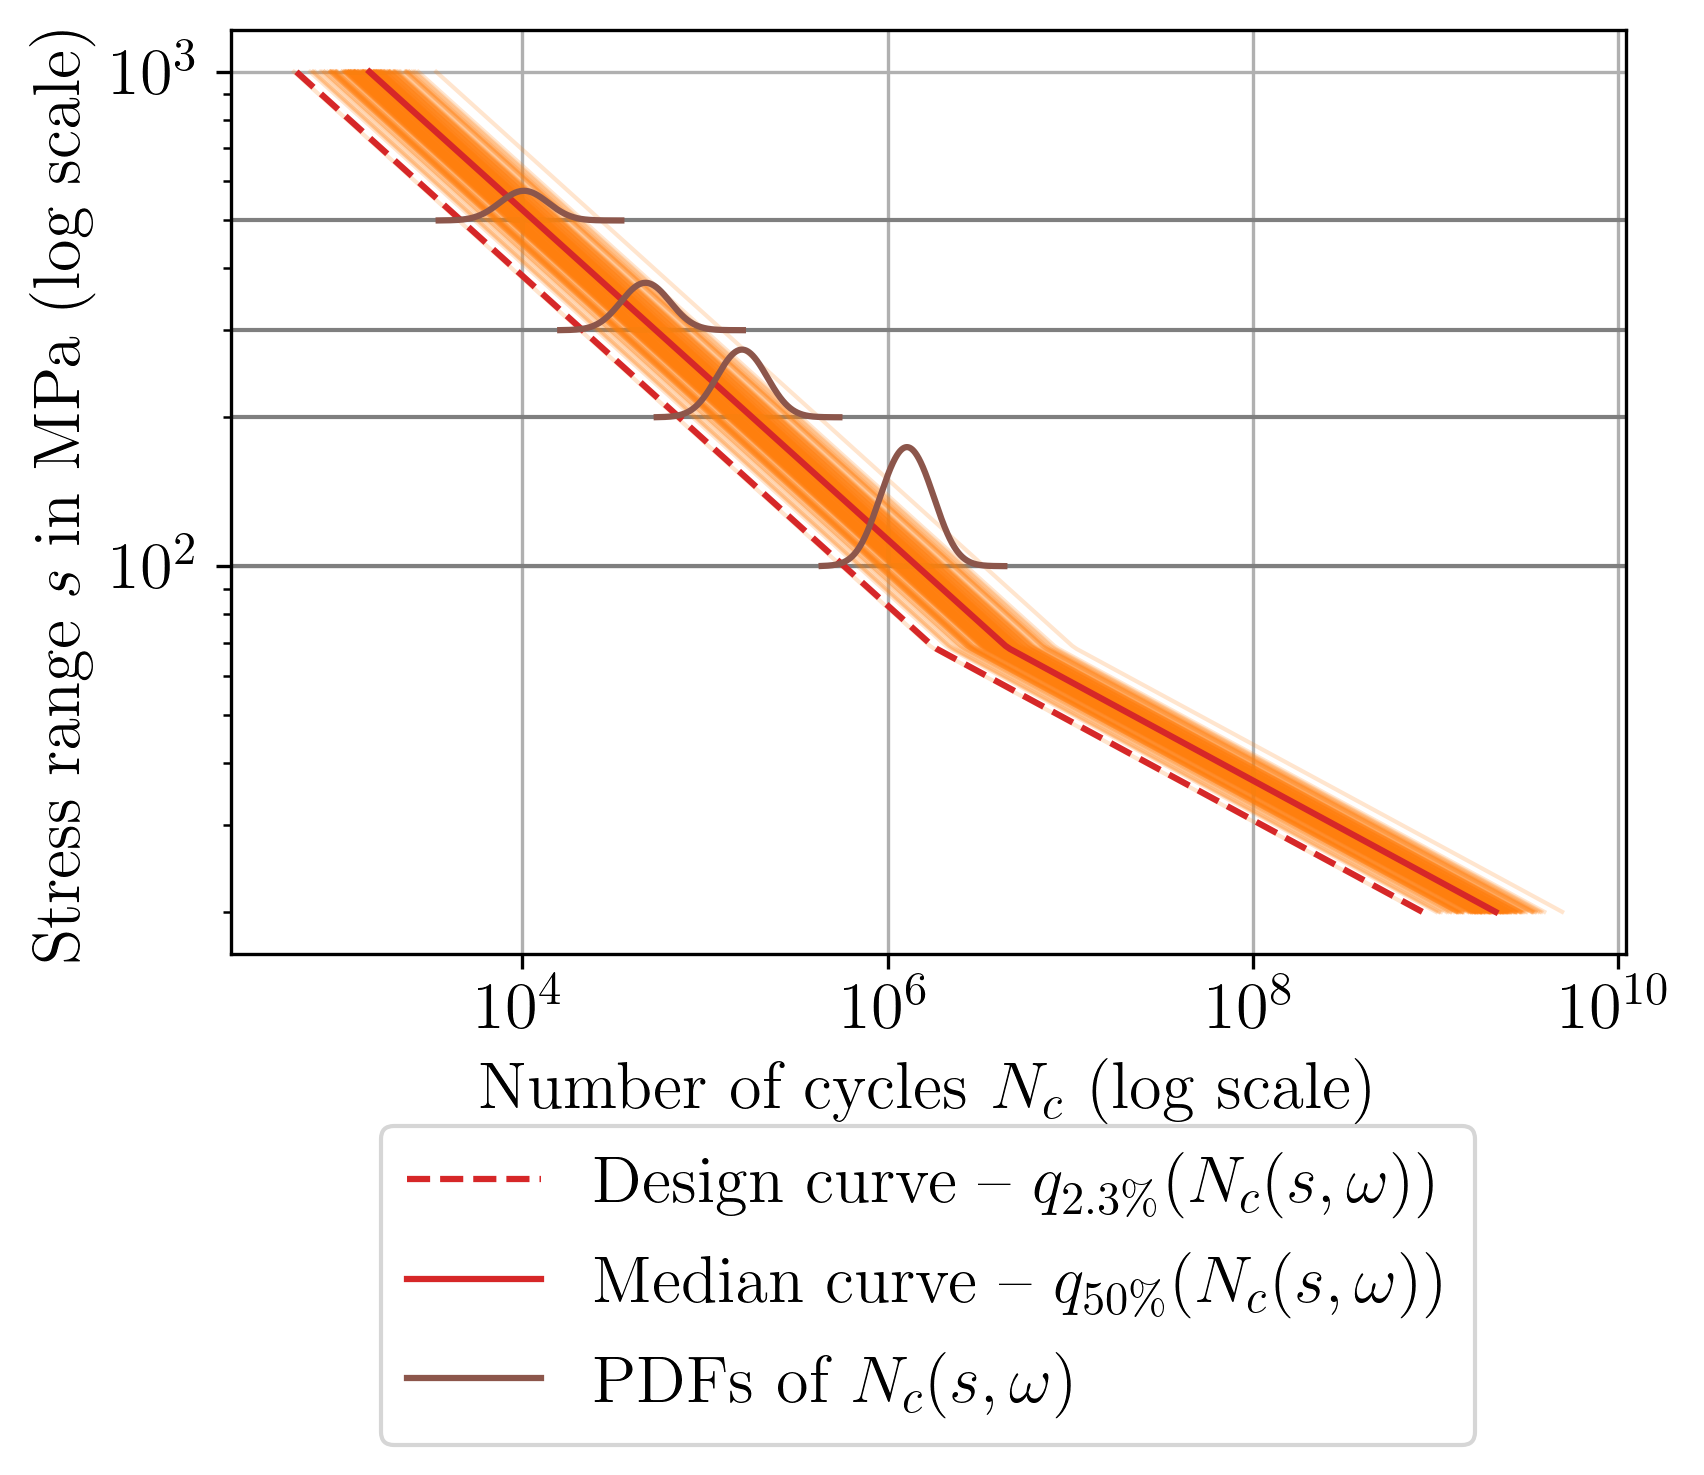
\includegraphics[width=0.6\textwidth]{../numerical_experiments/chapter2/figures/probabilistic_fatigue.png}
    \caption{Illustration of a probabilistic S-N curve according to the model defined in \citet{guede_2007}.}
    \label{fig:probabilistic_SN}
\end{figure}


%============================================================%
%============================================================%
\section{Conclusion}
%============================================================%
%============================================================%

This chapter proposed an overview of OWT modeling and design. 
It introduced some concepts related to the description and simulation of metocean conditions. 
The impact of the wake on the performance and on unsymmetrical fatigue loading was also explained.  
Then, the different theories considered in OWT modeling were introduced such as aerodynamics, hydrodynamics, structural dynamics and control. 
A variety of software implementations exist for OWT simulation, but special attention was brought to DIEGO, the numerical model developed by EDF R\&D which is used in the present work. 
%As a perspective, uncertainty quantification could benefit from the different fidelities proposed to model OWT systems presenting very nonlinear transient phases. 

To understand the design of OWTs, the most common technologies of bottom-fixed and floating turbines were presented. 
Then, a focus on a few critical topics to be considered during design and exploitation was proposed. 
In light of the previous elements, the variables considered random in this work were listed with a particular focus on probabilistic fatigue damage assessment.   

This growing industry faces various challenges, for example, related to the massive use of primary commodities, the cohabitation of offshore dynamic structures with an ecosystem, composite materials recycling, etc. 
UQ is a tool for understanding some of these problems, however, many uncertainties are hard to characterize and quantify. 
For example, manufacturing quality issues were recently revealed by Siemens Gamesa\footnotemark~regarding wrinkles on the surface of some blades, illustrating the considerable uncertainties present in wind energy. 


\footnotetext{L. Pitel and R. Millard. (August 7, 2023). Siemens Energy warns of €4.5bn loss from ailing wind turbine division. \textit{Finacial Times}. \url{https://www.ft.com/content/df8947cd-4bab-46ff-804e-b28de4b5a0f0}}

